\section{Validation}
% To validate the proposed method, the kinematic and dynamic regressions are tested in several simulation scenarios. Two simulators were used to generate the test cases: a planar PCS dynamic simulator and a planar Piecewise Affine Curvature (PAC) kinematic simulator. These simulators render videos of soft robot trajectories (see Fig. \ref{fig:pcsregression:cv_sequence}) to be used as input of the method's pipeline. 
% In the end, the quality of the kinematic and dynamic models is assessed by comparing the estimated poses from both models with the ground truth. The following subsections provide additional details and the results.
To validate the proposed approach, we verify the kinematic and dynamic regression algorithms separately.
We test the kinematic fusion algorithm on simulated continuum soft robots that behave according to the \gls{PCS} and \gls{PAC} model.
Subsequently, we compare the dynamic prediction performance of the proposed method against multiple \gls{ML} baseline methods on various \gls{PCS} soft robots.
Finally, we demonstrate how the regressed methods can be used in a plug-and-play fashion within a closed-form, model-based setpoint regulation framework.


\subsection{Experimental Setup}

% To evaluate the robustness of the constant strain assumption in the models, a second planar simulator with distinct kinematics was used. It implements piecewise affine curvature (PAC) \citep{stella2023piecewise}\citep{stella2022experimental}, in which the curvature of each segment $c_i(t)$ is no longer constant but rather affine in space,
% \begin{align}
%     c_i(t) = c_{0,i}(t) + c_{1,i}(t)s \,,
% \end{align}
% where $c_{0,i}$ and $c_{1,i}$ are the zero-order and first-order terms that define the curvature. The axial and shear strains are still considered constant in each segment. This simulator was used to generate \textbf{Case 6}, a one-segment PAC soft manipulator. Details on the manipulators used for the test cases are displayed in Table \ref{table:manipulator_params}.

% \begin{table}[htbp]
% \centering
% \caption{Segment lengths of the manipulators used in the experiments. All segments have a constant circular cross-section with radius $r=0.02 \, \mathrm{m}$.}
% \label{table:manipulator_params}
% \begin{tabular}{cc}
% \hline
% Case & Segment lengths [m] \\ \hline
% \textbf{1}, \textbf{4} & $L=[0.1]$           \\/
% \textbf{2}    & $L=[0.07;0.1]$      \\
% \textbf{3}    & $L=[0.05;0.1;0.06]$ \\
% \textbf{5}    & $L=[0.15]$              \\ \hline
% \end{tabular}
% \end{table}

% Cases 1, 2 and 4 served to validate the method end-to-end, whereas Cases 3 and 5 were used to test only the kinematic fusion part.

% \begin{figure*}[h!]
%     \centering
%     \subfloat[Case 1 (1-segment)\label{1a}]{%
%       \includegraphics[width=0.33\linewidth]{figures/distance_plot.pdf}}
%     \subfloat[Case 2 (2-segment)\label{1b}]{%
%        \includegraphics[width=0.33\linewidth]{figures/distance_plot_two_segments.pdf}}
%        %\\
%     \subfloat[Case 3 (3-segment)\label{1c}]{%
%         \includegraphics[width=0.33\linewidth]{figures/distance_plot_three_segments.pdf}}

%     \caption{Average strain distances between pairs of adjacent segments for the test cases generated using the PCS simulator. The poses of 20 cross-sections along the manipulators are tracked, resulting in 19 pairs of segments to be evaluated for strain similarity. The threshold is represented with a dashed line and the background shading marks the resulting segments (separate segments are shaded with a different colour).}
%     \label{fig:pcsregression:distances_pcs}
% \end{figure*}

\subsubsection{Evaluation Cases}
\paragraph{Cases 1-3 (1-3S PCS)}
These cases consider one-segment, two-segment, and three-segment planar \gls{PCS} soft robots ($n_\mathrm{s} \in \{ 1, 2, 3 \}$), respectively, with configurations $q \in \mathbb{R}^{n_\mathrm{q}}$ where $n_\mathrm{q} \in \{3, 6, 9 \}$ and actuation  $\tau \in \mathbb{R}^3, \mathbb{R}^6, \mathbb{R}^9$, assuming full actuation.

\paragraph{Case 4 (1S PCS H-SH)}
This case is a one-segment \gls{PCS} robot with high shear stiffness, three orders of magnitude larger than in \emph{Case 1}.

\paragraph{Case 5 (2S PCS H-AX/SH)}
This case is a two-segment \gls{PCS} robot, where the \nth{1} segment has a significantly increased axial stiffness and \nth{2} segment an increased shear stiffness w.r.t \emph{Case 2}.

\paragraph{Case 6 ( 1S PAC)} This case considers a one-segment \gls{PAC} robot whose curvature can be described by an affine function~\citep{stella2023piecewise}.

% \textbf{Case 1: 1S PCS}, \textbf{Case 2: 2S PCS} and \textbf{Case 3: 3S PCS} represent one-, two- and three-segment planar \gls{PCS} soft robots ($n_\mathrm{s} \in \{ 1, 2, 3 \}$), respectively, with configurations $q \in \mathbb{R}^{n_\mathrm{q}}$ where $n_\mathrm{q} \in \{3, 6, 9 \}$ and actuation  $\tau \in \mathbb{R}^3, \mathbb{R}^6, \mathbb{R}^9$, assuming full actuation.
% \textbf{Case 4: 1S PCS H-SH} is a one-segment \gls{PCS} robot with high shear stiffness three orders of magnitude larger than in \emph{Case 1}.
% \textbf{Case 5: 2S PCS H-AX/SH} is a two-segment \gls{PCS} robot, where the \nth{1} segment has a significantly increased axial stiffness and \nth{2} segment an increased shear stiffness w.r.t \emph{Case 2}.
% \textbf{Case 6: 1S PAC} considers a one-segment \gls{PAC} robot whose curvature can be described by an affine function~\citep{stella2023piecewise}.


\subsubsection{Dataset Generation}
In order to illustrate the end-to-end nature of our proposed method, we generate the datasets as short video sequences of the soft robot's movement. 
Therefore, we mimic a camera placed parallel to the robot's plane of motion to capture the soft robot's ground-truth dynamics.
At each time step, we render an image of the soft robot that contains $N=21$ equally distant, visually salient features. In the real world, this could be achieved by attaching markers to the soft robot that allow tracking of points along the backbone across time~\citep{stella2022experimental}.
We simulate the robot's ground-truth dynamics using the planar \gls{PCS} simulator presented in \citep{stolzle2024experimental}.

For Cases 1 to 4, we include eight trajectories with randomly sampled initial conditions in the training set. We consider stepwise actuation sequences for which we randomly sample a torque every \SI{10}{ms}. Each trajectory produces a \SI{0.5}{s} video captured at \SI{1000}{Hz}. For \emph{Case 6}, since the PAC simulator only accounts for kinematics, we generate an image sequence featuring the robot in $500$ randomly selected configurations.
As the test set, an additional trajectory with \SI{7}{s} duration is generated by applying a sinusoidal actuation sequence with $\tau = a_1\sin{(\omega_1 t)} + a_2\cos{(\omega_2 t)} \in \mathbb{R}^{n_\mathrm{q}}$, where $a_1$ and $a_2$ are random amplitudes, and $\omega_1$ and $\omega_2$ are random frequencies.
%To evaluate the accuracy, another trajectory is used. In this case, to ensure continuity and realism between frames, this test trajectory is created by linearly interpolating between two random configurations.

\subsubsection{Backbone Shape Detection from Images}
To apply our proposed model identification method, we first extract the motion of several Cartesian-space samples along the robot's backbone.
As we consider a planar problem setting and rendered images of the soft robot's shape, the goal is to extract the SE(2) poses of $N$ cross-sections along the robot.
To satisfy the assumption behind the \emph{Kinematic Fusion} algorithm, the number of extracted poses $N$ should be significantly larger than the expected number of \gls{PCS} segments required to model the robot's behavior accurately: $N \gg n_\mathrm{s}$.
% A camera is placed parallel to the robot's plane of motion and records several trajectories of the robot. The goal is to extract the poses of $N$ equally distant cross-sections along the robot. The value of $N$ should be significantly larger than the expected number of segments required to model the robot's behavior accurately.% videos are analyzed using the OpenCV library in Python to extract the poses of $N$ equally distant cross-sections along the robot. The value of $N$ should be significantly larger than the expected number of segments required to model the robot's behavior accurately.
%
% Fig. \ref{fig:pcsregression:cv_sequence} illustrates the steps involved in this process. 
We leverage the \emph{OpenCV} library for detecting the soft robot contour (\texttt{findContours}) and extracting pose measurements along its backbone (\texttt{minAreaRect}).
Each frame is binarized, and the contours of cross-sections are identified.
This allows the extraction of the center position $(p_{\mathrm{x},j},p_{\mathrm{y},j})$ and orientation $\theta_j$ of each cross-section (also referred to as \emph{marker}).
As in our case, the markers are equally distant, we compute, without loss of generality, the backbone abscissa as $s_j= \frac{j-1}{N} L$. % , where $L$ is assumed to be the known total length of the soft robot backbone in an undeformed configuration.
% Each of the $N$ points is marked with visually salient features, which allows the extraction of their center position $(p_x,p_y)$ and orientation $\theta$.
%Each of the contours is then fitted with a minimum area rectangle around it, which allows to extract its center position $(p_x,p_y)$ and orientation $\theta$. 
For $T$ video frames, this results in a time sequence of SE(2) poses $\{\chi (1),...,\chi (T) \}$,  $\chi_j = \begin{bmatrix}
    \chi_1^\top \dots \chi_N^\top
\end{bmatrix}^\top \in \mathbb{R}^{3N}$, and $j \in \{ 1, \dots, N \}$.
We leverage a Savitzky-Golay filter (\nth{3}-order, window length $25$) to estimate the associated pose velocities $\dot{\chi}$ and velocities $\ddot{\chi}$.

% \begin{figure}[htbp]
% \centerline{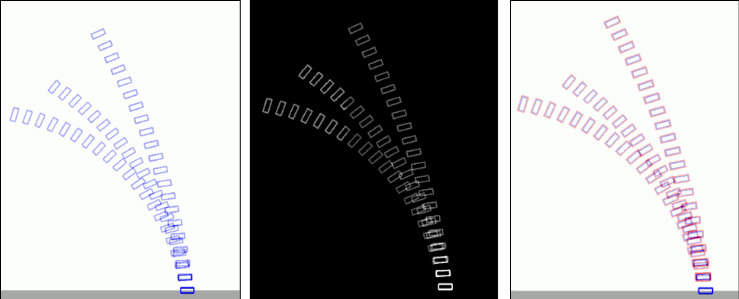
\includegraphics[scale=.35]{figures/cv_seq.png}}
% \caption{Image analysis pipeline to obtain the Cartesian pose of $N$ cross-sections, applied to a sequence of video frames. From left to right: 1) original image; 2) binarized image; 3) original image superimposed with the fitted rectangles.}
% \label{fig:pcsregression:cv_sequence}
% \end{figure}

\subsubsection{Evaluation metrics}
To evaluate the models quantitatively, we introduce position and orientation task space metrics. 
We use a Cartesian-space \gls{MAE} measuring the deviation of the estimated from the actual robot body shape, given by

\begin{equation}
\begin{split}
    % e_\mathrm{p}^{\mathrm{body}} =& \: \frac{1}{N T} \sum_{k=1}^T \sum_{i=1}^N \lVert \hat{p}_i(k) - p_i(k) \Vert_2,\\
    % e_{\theta}^{\mathrm{body}} =& \: \frac{1}{N T} \sum_{k=1}^T \sum_{i=1}^N | \hat{\theta}_i(k) - \theta_i(k) |,
     e_\mathrm{p}^{\mathrm{body}} = \sum_{k=1}^T \sum_{j=1}^N \frac{\lVert \hat{p}_j(k) - p_j(k) \Vert_2}{N T},
     \quad
    e_{\theta}^{\mathrm{body}} = \sum_{k=1}^T \sum_{j=1}^N \frac{| \hat{\theta}_j(k) - \theta_j(k) |}{N T},
\end{split}
\end{equation}
where 
% $\hat{p}_i(k) = \begin{bmatrix}
%     \hat{p}_{\mathrm{x},i}(k) & \hat{p}_{\mathrm{y},i}(k)
% \end{bmatrix}^\top \in \mathbb{R}^2$ 
$\hat{p}_i(k)$ and $\hat{\theta}_i(k) \in \mathbb{R}$ are the estimated position and orientation of point $i$ along the structure, respectively, while $p_i(k)$ and $\theta_i(k)$ are the ground-truth counterparts. These metrics give the average pose error across all $T$ frames of a trajectory and all $N$ cross-sections tracked along the robot, enabling a good evaluation of the kinematic model by capturing how well it represents the overall shape of the soft robot structure.

\begin{figure*}[ht]
    \centering
    \subfigure[2S PCS: Strain distances]{\includegraphics[width=0.49\textwidth,trim={5 5 5 5}]{pcsregression/figures/distance_plot_two_segments.pdf}\label{fig:pcsregression:results:kinematic_fusion:pcs_ns-2}}
    \subfigure[3S PCS: Strain distances]{\includegraphics[width=0.49\textwidth,trim={5 5 5 5}]{pcsregression/figures/distance_plot_three_segments.pdf}\label{fig:pcsregression:results:kinematic_fusion:pcs_ns-3}}\\
    \subfigure[1S PAC: Strain distances]{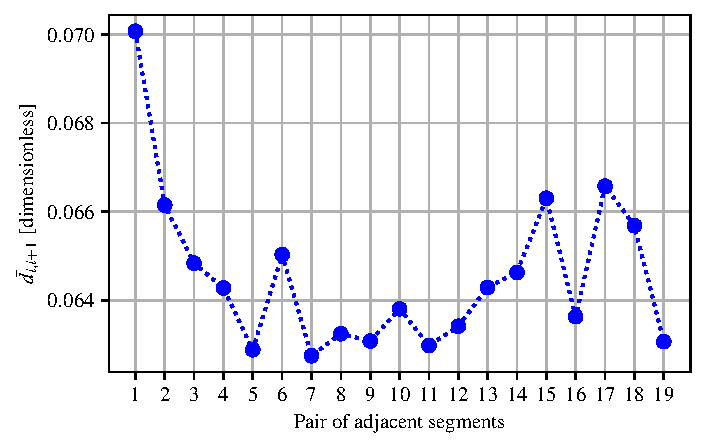
\includegraphics[width=0.46\textwidth,trim={5 5 5 5}]{pcsregression/figures/distance_plot_pac.pdf}\label{fig:pcsregression:distances_pac}}
    \subfigure[1S PAC: Kinematic Pareto Front]{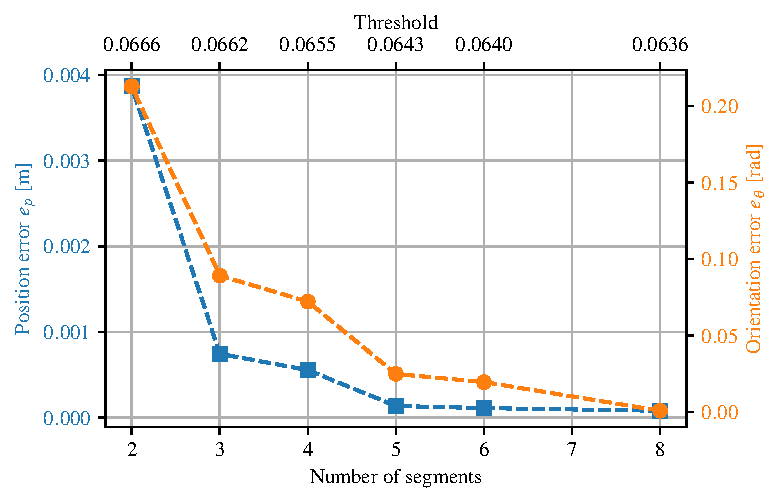
\includegraphics[width=0.50\textwidth,trim={5 5 5 5}]{pcsregression/figures/pareto_front_pac.pdf}\label{fig:pcsregression:pareto_front_pac}}
    \caption{
    Kinematic Fusion Results:
    \textbf{Panels (a) \& (b):} Average strain distances between pairs of adjacent segments for \emph{Cases 2 \& 3}. The poses of $20$ markers along the manipulators are tracked, resulting in $19$ pairs of segments to be evaluated for strain similarity. The threshold is represented by a dashed line, and the background shading marks the resulting segments (separate segments are shaded in different colors).
    \textbf{Panel (c):} Average strain distances between segments after the first iteration of the kinematic fusion algorithm for \emph{Case 6}. \textbf{Panel (d):} Pareto front that describes the trade-off between the DOF of the kinematic model (i.e., the number of segments) and the shape reconstruction error for \emph{Case 6}.
    The blue and orange lines represent the average kinematic body position error $e_\mathrm{p}^\mathrm{body}$ and the body orientation error $e_\theta^\mathrm{body}$, respectively.
    % Position ($\blacksquare$) and orientation ($\CIRCLE$) distributed errors as a function of the number of segments considered for the kinematic model in Case 6.
    The strain distance threshold $h$ that is used for separating segments is plotted on the upper x-axis.
    }\label{fig:pcsregression:results:kinematic_fusion}
\end{figure*}

In addition, we consider an end-effector Cartesian-space \gls{MAE} given by
\begin{equation}
    e_p^{\mathrm{ee}} = \frac{1}{ T} \sum_{k=1}^T \lVert \hat{p}_\mathrm{ee}(k) - p_\mathrm{ee}(k) \rVert_2,
    \quad
    e_{\theta}^{\mathrm{ee}}=\frac{1}{T} \sum_{k=1}^T | \hat{\theta}_\mathrm{ee}(k) - \theta_\mathrm{ee}(k) |,
\end{equation}
where $\hat{p}_\mathrm{ee}(k) = \hat{p}_{N}(k) \in \mathbb{R}^2$ and $\hat{\theta}_\mathrm{ee}(k) \in \mathbb{R}$ are the estimated end-effector position and orientation, respectively, with $p_\mathrm{ee}(k)$ and $\theta_\mathrm{ee}(k)$ being the ground-truth counterparts. 
This metric is particularly useful for assessing the obtained dynamic models with a control perspective, as the accuracy of the end-effector predictions is crucial for effective control in task space.
% For the kinematic model, once the final number of segments $m$ and their locations are determined, we retrieve for the test trajectory the configurations $\mathbf{q}_i(k)$ at each of the segments. Then, knowing the coordinate $s$ of each of the $N$ tracked points along the robot, the estimated positions and orientations are found using the forward kinematics in \eqref{eq:pcsregression:forward_kin_pcs}. For the dynamic model, after obtaining the final coefficients for the Lagrangian and damping effects, we can get the robot's equations of motion. Those are integrated with the initial conditions of the test trajectory to obtain the estimated configurations. The estimated positions and orientations are again found as above through forward kinematics.

\subsection{Kinematic Fusion Results}
\subsubsection{Cases 1, 2, and 3}
% The kinematic fusion procedure was first tested for three instances of the planar PCS simulator: a one-, two- and three-segment manipulators (Cases 1, 2 and 3). %The video processing step extracts the poses of the 20 cross-sections and a 20-segment kinematic model is initialized. 
Figs. \ref{fig:pcsregression:results:kinematic_fusion:pcs_ns-2} \& \ref{fig:pcsregression:results:kinematic_fusion:pcs_ns-3} presents the average strain distances between the adjacent segment pairs for \emph{Cases 2-3}, as the result of the first and final iteration of the kinematic fusion algorithm. 
The plots for Cases 2 and 3 reveal one and two peaks, respectively, revealing where we need to separate segments in the kinematic model.
% In contrast, the smaller magnitude of the distance metric in Case 1, when compared to the other cases, indicates that the entire robot can be represented by a single segment with constant strain. 
The strain distance threshold $h$ is a hyperparameter that trades off model complexity with model accuracy.
For common soft robots that exhibit a \gls{PCS}-like behavior, we recommend choosing $h$ such as that the segmented model exhibits isolated peaks in the strain distance metric, as visible in Fig.~\ref{fig:pcsregression:results:kinematic_fusion}.
The number of segments and respective lengths for the resulting models obtained with a threshold of $h=0.2$ are presented in the third column of Table \ref{tab:pcsregression:results_kin_reg_pcs}, and by comparing to the second column, it is easily visible that our algorithm almost perfectly identified the segment lengths. 
% Note that these models are final because, for Cases 2 and 3, the updated strain trajectories for the newly defined segments are no longer sufficiently similar for further merging. Also, for Case 1 no additional merging is possible since we already reached one single segment.
%
% The distributed task-space errors between the resulting models and the ground truth is also evaluated. Knowing the final number of segments and their lengths, we determine the configurations $\mathbf{q}_i(k)$. Then, using the forward kinematics in \eqref{eq:pcsregression:forward_kin_pcs}, we obtain the estimated positions and orientations for the 20 tracked points along the robot. The results for these three cases are summarized in the first three rows of Table \ref{tab:pcsregression:results_kin_reg_pcs}.
As a consequence of the correct identification of the number of segments and segment lengths, the identified kinematic model also accurately captures the shape of the robot with the position errors below \SI{0.2}{\percent} of the robots' length, as it can be seen from the body shape reconstruction errors stated in the first three rows of Table \ref{tab:pcsregression:results_kin_reg_pcs}.
We remark that the error can be further reduced by using a finer discretization of backbone pose markers (i.e., increasing $N$).
% The evaluation of the kinematic fusion algorithm for Cases 4 \& 5 is not necessary as it would give very similar results as reported for Cases 1 \& 2.

\begin{table}[htbp]
\centering
% \renewcommand{\arraystretch}{1.3} % Increase space between rows
\caption{Kinematic fusion results: The second and third columns contain the actual and estimated segment lengths, respectively. The Cartesian pose error between the actual and estimated backbone shape is stated in the third and fourth columns, respectively. \emph{Case 6} represents a one-segment \gls{PAC} soft robot of total length \SI{150}{mm} and can be, therefore, not be represented with a (one-segment) \gls{PCS} model.}
\label{tab:pcsregression:results_kin_reg_pcs}
\setlength\tabcolsep{3.0pt}
\begin{small}
    \begin{tabular}{ccccc}\toprule
    \textbf{Case} & \begin{tabular}[c]{@{}c@{}}\textbf{Actual segment}\\ \textbf{lengths} $\mathbf{L}$ \textbf{[mm]}\end{tabular} & \begin{tabular}[c]{@{}c@{}}\textbf{Estimated segment}\\ \textbf{lengths} $\mathbf{\hat{L}}$ \textbf{[mm]}\end{tabular} & $\mathbf{e_\mathrm{p}^{\mathrm{body}}}$ \textbf{[mm]} & $\mathbf{e_{\theta}^{\mathrm{body}}}$ \textbf{[rad]} \\ \midrule
    \textbf{1: 1S PCS} & $[100]$ & $[100]$ & $0.082$ & $6.38\times 10^{-3}$ \\
    \textbf{2: 2S PCS} & $[70, 100]$ & $[68, 102]$ & $0.240$ & $1.15\times 10^{-2}$               \\
    \textbf{3: 3S PCS} & $[50, 100, 60]$ & $[52.5, 94.5, 63.0]$ & $0.210$ & $9.67\times 10^{-3}$ \\
    \textbf{6: 1S PAC} & $[150]$ & $[7.5, 105.0, 37.5]$ & $0.746$ & $8.92\times 10^{-2}$  \\
    \bottomrule
    \end{tabular}
\end{small}
\end{table}

% The kinematic fusion was able to retrieve models that almost exactly match the manipulators used in the simulation. However, for Cases 2 and 3, the segments' lengths deviate slightly from the true ones (see second column of Table \ref{table:manipulator_params}). This is a consequence of the number of cross-sections tracked along the robots. Increasing this number would result in finer discretization and a closer approximation. Nonetheless, the position errors of the resulting models fall under 0.2\% of the robots' lengths.

\subsubsection{Case 6}
Even though the kinematics of many continuum soft robotic manipulators can be described by \gls{PCS}/\gls{PCC} kinematics, other continuum soft robots can only be described by piecewise constant models in the limit $N \to \infty$ as they exhibit polynomial curvature~\citep{della2019control, stella2022experimental} or even more generally \gls{GVS}~\citep{boyer2020dynamics}.
This is particularly the case when external or gravitational forces dominate the elastic and actuation forces~\citep{della2023model}.
In order to verify that our approach is also able to identify effective models in such situations, we test the kinematic fusion algorithm on the case of an affine curvature robot~\citep{stella2023piecewise} and plot the resulting average strain distances in Fig.~\ref{fig:pcsregression:distances_pac}.
Indeed, the strain distance plot no longer exhibits clear, isolated peaks (i.e., a single solution). Therefore, we formulate a Pareto front in Fig.~\ref{fig:pcsregression:pareto_front_pac} (by varying the strain distance threshold $h$) that describes the tradeoff between the number of \gls{PCS} segments (i.e., the \gls{DOF} of the kinematic model) and the shape reconstruction accuracy. Analyzing and exploiting this tradeoff allows the user to choose their \emph{sweetspot} between model complexity and performance.
In this case, we find that three segments represent a suitable compromise between model complexity and shape reconstruction accuracy, as it exhibits a position error of only \SI{0.5}{\percent} of the robot's length.

% We evaluate the robustness of the method with the PAC simulator, which no longer implements the constant bending assumption of the PCS model. The average strain distances for the initial 19 pairs of segments are presented in Fig. \ref{fig:pcsregression:distances_pac}.


% Contrary to the results for the previous test cases, the plot does not make clear the exact locations where to merge segments. In this situation, we could think of the threshold as a hyperparameter and evaluate the quality of the models resultant from different values of $h$. Figure \ref{fig:pcsregression:pareto_front_pac} shows the position and orientation errors as a function of the obtained number of segments, for several values of threshold. The choice for the final kinematic model depends on how the user wants to balance model complexity and shape reconstruction accuracy. For this case, we choose as the final model the one that maximizes the decrease in error over an increase in complexity (i.e., number of segments), which corresponds to the model with three segments. We can see that the 3-segment model exhibits a distributed position error of 0.5\% of the robot's length, which verifies that this kinematic parametrization is suitable to approximate the robot's behaviour.

% \begin{figure}[htbp]
%     \centering
%     \subfloat[Position error\label{1a}]{%
%       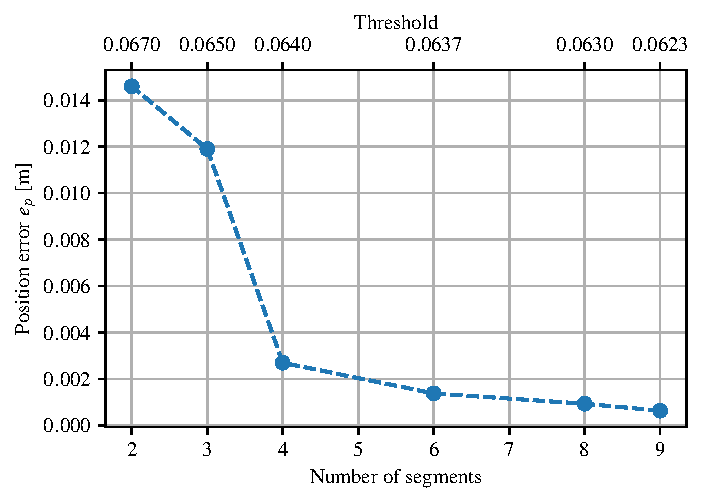
\includegraphics[width=0.8\linewidth]{pcsregression/figures/pareto_front_pac_pos.pdf}}
%     \\
%     \subfloat[Orientation error\label{1b}]{%
%        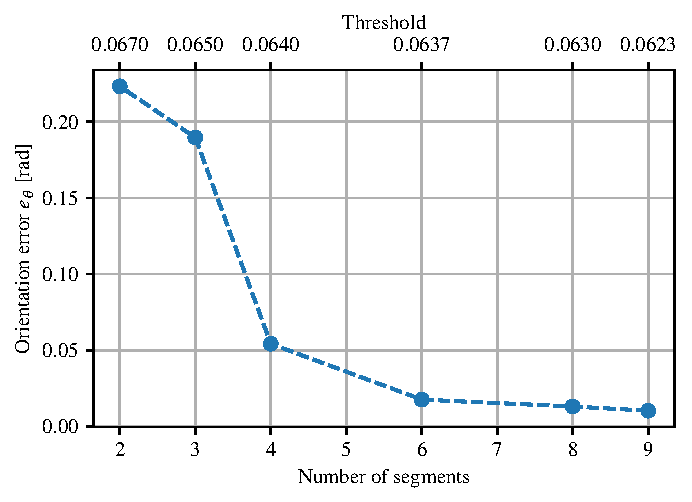
\includegraphics[width=0.8\linewidth]{pcsregression/figures/pareto_front_pac_ori.pdf}}
%        %\\

%     \caption{Average strain distances between pairs of adjacent segments for tasks generated using the PCS simulator. The poses of 20 cross-sections along the manipulators are tracked, resulting in 19 pairs of segments to be evaluated for strain similarity.}
%     \label{fig:pcsregression:pareto_front_pac}
% \end{figure}

% This 4-segment model was evaluated on the test trajectory and the task space errors are presented in the final row of Table \ref{table:results_kin_reg_pcs}. The positional error corresponds to 4\% of the robot's length, which verifies that this kinematic parametrization is suitable to approximate the robot's behavior.

\subsection{Dynamic Model Identification Results}

\subsubsection{Verification of Dynamical Regression}
We verify the dynamical regression algorithm on one and two-segment \gls{PCS} robots (i.e., Cases 1 \& 2), both with and without measurement noise.
After regressing the dynamic parameters on the training set, we perform a rollout on the test set and compare the resulting predicted trajectory with the ground truth.
To confirm that the dynamic regression is also effective when applied to real-world data, we apply in some experiments Gaussian noise that mirrors measurement noise as we would encounter it for motion capture data, computer vision detection errors, etc. to the poses included in the training set (i.e., $\Tilde{\chi} = \chi + \mathcal{N}(0, \sigma_\mathrm{n}))$.
For \emph{Case 1}, we sample the noise from a normal distribution with standard deviations \SI{0.5}{mm} and \SI{1}{\degree} for the position and orientation measurements, respectively.
Analog, we define the standard deviation of the noise for \emph{Case 2} as \SI{0.1}{mm} and \SI{0.5}{\degree}.

The results are reported in Tab.~\ref{tab:pcsregression:dyn_results} (top four rows), and the rollouts of Cases 1 \& 2 are included in Figs.~\ref{fig:pcsregression:predict_ns-1}-\ref{fig:pcsregression:predict_ns-2}. We also present a sequence of stills of the rollout of \emph{Case 2} in Fig.~\ref{fig:pcsregression:still_seq}.
We conclude that even though the dynamical parameters are regressed on only \SI{4}{s} of robot motion data, the dynamical predictions are extremely accurate on the long horizon of \SI{7}{s} (most control algorithms such as \gls{MPC} operate on a much smaller horizon). The position error for the experiments not involving noise stays below \SI{5}{\percent} in both cases.
When noise is present in the training data, the position error is roughly tripled. Still, we observe that the error is mostly related to the transient terms and the model converges during the slower sequences of the trajectory to the ground truth. Most importantly, the learned model, even when trained on noisy data, remains stable, as shown in Fig.~\ref{fig:pcsregression:predict_ns-2}.

\subsubsection{Verification of Strain Sparsification}
Next, we verify that the strain sparsification algorithm can detect and eliminate strains that do not have a significant effect on the dynamics and can be, therefore, neglected to reduce the model complexity.
For this purpose, we apply the integrated \emph{Dynamic Regression and Strain Sparsification} algorithm to \emph{Cases 4 \& 5}, which exhibit no shear strain and no axial strain (\nth{1}-segment) \& no shear strain (\nth{2}-segment), respectively.
We define the maximum elastic and shear modulus as $E^\mathrm{max} = \SI{100}{MPa}$ which leads to the stiffness thresholds for each segment $K_j^\mathrm{max} = \mathrm{diag}(\SI{12.6}{Nm^2}, \SI{168}{N}, \SI{126}{kN})$.
For example, in \emph{Case 4}, after determining the dynamic parameters during the first iteration, the algorithm detects that the estimated shear stiffness $\hat{K}_\mathrm{sh} = \SI{1200}{N} > K_\mathrm{sh}^\mathrm{max} = \SI{168}{N}$. Therefore, the shear strain is eliminated from the dynamic model, and the dynamic parameters are newly regressed during the next iteration.
Similarly, the algorithm correctly neglects the axial strain for the \nth{1} segment and the shear strain for the \nth{2} segment of \emph{Case 5}.
We visualize the test set rollouts for \emph{Cases 4 \& 5} in Fig.~\ref{fig:pcsregression:results:strain_sparsification} and report the error metrics in the last three rows of Tab.~\ref{tab:pcsregression:dyn_results}.
The results show that in \emph{Case 4}, the model without shear even exhibits a slightly smaller position error than the model that includes all strains. A possible explanation could be that with the Lagrangian being parametrized by fewer basis functions, the coefficients for the remaining strains can be more accurately regressed.
If we compare \emph{Case 2} and \emph{Case 5} (both two-segment \gls{PCS} robots), \emph{Case 5} exhibits significantly increased position and orientation errors. Still, we notice that the model predictions are usable, in particular for shorter horizons.

% We now present and discuss the results of the dynamic model identification procedure. The procedure is the same across all the tested manipulators. From the kinematic fusion step, we retrieve the kinematic model (with generic $m$-segments) and the respective configurations $\mathbf{q}(k) \in \mathbb{R}^{3m}$ for each of the 4000 time steps captured throughout the eight generated trajectories. The velocity $\dot{\mathbf{q}}(k)$ and acceleration $\ddot{\mathbf{q}}(k)$, also required for the regression, are numerically approximated using the Savitzky-Golay filter \citep{savitzky_smoothing_1964}, with a window length of 25 and a third-order polynomial. We gather the basis functions of the $m$-segment PCS Lagrangian (considering all three strains per segment) and initialize the diagonal damping matrix $\mathbf{D} \in \mathbb{R}^{3m\times 3m}$ to be also identified. After running the least-squares regression and strain sparsification iteratively, we compute the Euler-Lagrange equations with the obtained model and retrieve the robot's equations of motion. We then simulate the model for the sinusoidal validation trajectory, using a Tsitouras 5(4) integrator \citep{tsitouras_rungekutta_2011} and a time-step of 0.1 $\mathrm{ms}$.
% \subsubsection{Case 1}
% The Lagrangian of a one-segment PCS manipulator contains 51 basis functions. To those, we also add the 3 damping terms, yielding 54 coefficients to be identified.

\begin{table}[htbp]
\centering
% \renewcommand{\arraystretch}{1.2}
\caption{Dynamic regression results: End-effector position and orientation errors $\mathbf{e_\mathrm{p}^{\mathrm{ee}}}, \mathbf{e_{\theta}^{\mathrm{ee}}}$ for the obtained dynamic models evaluated on the \SI{7}{s} sinusoidal test set trajectory. In some cases, we add artificial measurement noise to the training data. For \emph{Case 4}, we present two variants of the learned model: in the first instance, we report the performance of a model that neglects strains as suggested by the dynamic sparsification algorithm. For completeness, we furthermore also state the performance of a model that considers all strains. In \emph{Case 5}, the \nth{1} segment only exhibits bending and shear strains (i.e, no axial strain), and the \nth{2} segment only exhibits bending and axial strains (i.e., no shear strain)}
\label{tab:pcsregression:dyn_results}
\setlength\tabcolsep{2pt}
\begin{small}
\begin{tabular}{c c c c c }
    \toprule
    \textbf{Case} & \textbf{Meas. Noise} & \textbf{Model Strains}     & $\mathbf{e_\mathrm{p}^{\mathrm{ee}}}$ \textbf{[mm]} & $\mathbf{e_{\theta}^{\mathrm{ee}}}$ \textbf{[rad]} \\
    \midrule
    1: 1S PCS & \xmark                     & All                & $4.89$    & $0.113$             \\ 
    1: 1S PCS & \cmark                        & All                & $13.7$    & $0.307$             \\ 
    \midrule
    2: 2S PCS & \xmark                     & All                & $5.22$    & $0.138$             \\
    2: 2S PCS & \cmark                        & All                & $16.8$    & $0.135$             \\ 
    \midrule
    4: 1S PCS H-SH & \xmark & No shear                     & $4.57$    & $0.099$                                 \\ 
    4: 1S PCS H-SH & \xmark & All                & $5.14$    & $0.116$ \\
    \midrule
    5: 2S PCS H-AX/SH & \xmark & (\cmark, \cmark, \xmark, \cmark, \xmark, \cmark) & $17.9$ & $0.305$\\
    \bottomrule
\end{tabular}
\end{small}
\end{table}

% After performing the least-squares regression, we inspect the estimated stiffness and compare it to the maximum defined stiffness. We choose $E^{\text{max}}=100 \,\mathrm{MPa}$ and $G^{\text{max}}=0.1 \,\mathrm{MPa}$, which are in line with the range of soft materials typically used \citep{gariya_review_2021}. For the cross-section area $A_c$ and second moment of inertia $I_c$, we assumed a constant circular cross-section along the segment, with the same radius defined in the simulator. With the above parameters, the maximum stiffness is
% \begin{equation}\label{eq:pcsregression:max_stiffness}
%     \begin{aligned}
%         K^{\text{max}} &=\mathrm{diag} \begin{bmatrix}
%         k_{\text{be}}^{\text{max}} & k_{\text{sh}}^{\text{max}} & k_{\text{ax}}^{\text{max}}   
%         \end{bmatrix} \\
%         &= \mathrm{diag}\begin{bmatrix}
%             1.26\times 10^1 & 1.68 \times 10^2 & 1.26\times10^5
%         \end{bmatrix} \,.
%     \end{aligned}
% \end{equation}

% The estimated stiffness obtained from the regression is
% \begin{align}
%     \hat{K} = \mathrm{diag} \begin{bmatrix}
%     1.20\times 10^{-3} & 1.55 \times 10^0 & 1.14\times10^1 
% \end{bmatrix}\,.
% \end{align}

% Since all values are below the maximum, no strains will be neglected and the dynamic model is final.

% To evaluate the robustness of the method, we also corrupted the videos by adding zero-mean Gaussian noise to the position and orientation of each of the 20 cross-sections along the robot. Specifically, noise with a standard deviation of $5 \times 10^{-4} \, \mathrm{m}$ was added to both the $x$- and $y$-position measurements, while a standard deviation of $1\, \mathrm{deg}$ was applied to the orientation. Figure \ref{fig:pcsregression:predict_ns-1} shows the comparison between the models trained with and without noise. 

\begin{figure*}[htbp]
    \centering
    \subfigure[Configurations]{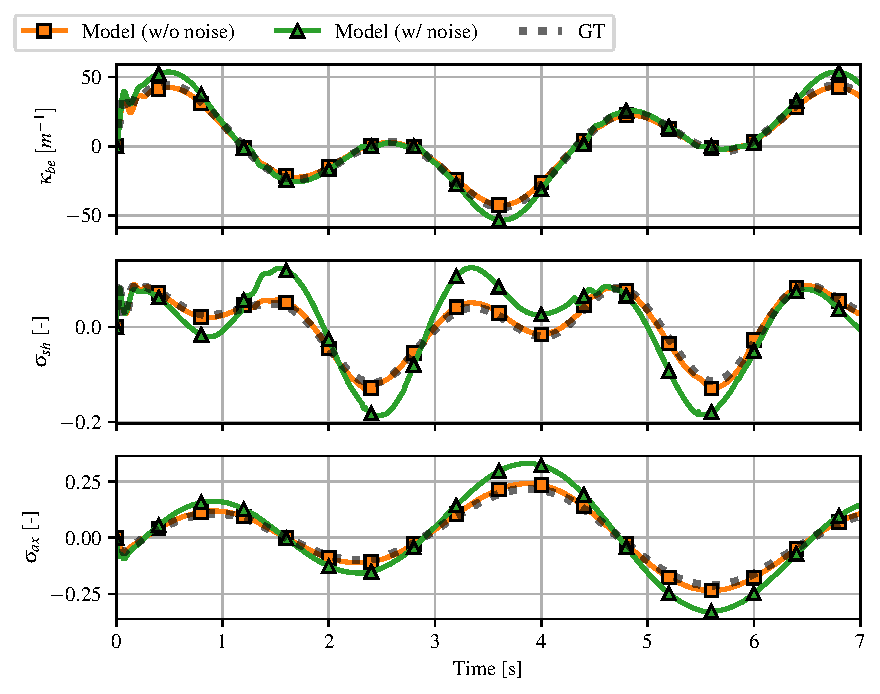
\includegraphics[width=0.49\linewidth]{pcsregression/figures/pcs_ns-1/ns-1_configuration_plots.pdf}\label{fig:pcsregression:predict_ns-1_subfig-1}}
    \subfigure[End-effector pose]{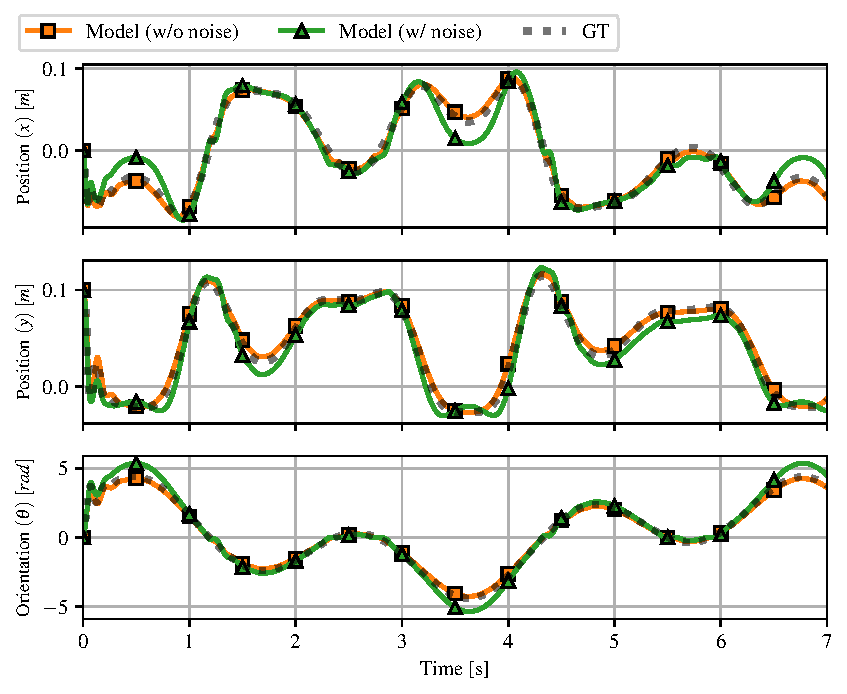
\includegraphics[width=0.47\linewidth]{pcsregression/figures/pcs_ns-1/ns-1_ee_comparison_plots.pdf}\label{fig:pcsregression:predict_ns-1_subfig-2}}

    \caption{Verification of the model obtained for Case 1 on a sinusoidal trajectory. The dotted line denotes the ground-truth (GT) trajectory, while the green and orange lines correspond to the models trained with and without noise, respectively.}
    \label{fig:pcsregression:predict_ns-1}
\end{figure*}

% The task-space error analysis, reported on Table \ref{tab:pcsregression:dyn_results}, show that the model trained without noise is able to give very accurate predictions, with the end-effector position error being under $5\%$ of the robot's length. The model trained from noisy data can still provide reasonable predictions, even though the position error increases to $1.37\, \mathrm{cm}$ and the orientation error rises to $0.3\, \mathrm{rad}$. 

% \begin{table*}[htbp]
% \centering
% \renewcommand{\arraystretch}{1.5}
% \caption{Error metrics for Cases 1, 2, and 4. Distributed task-space errors and end-effector errors are reported for both position and orientation. Cases 1 and 2 include results with and without added noise during training.}
% \label{tab:pcsregression:dyn_results}
% \begin{tabular}{|>{\centering\arraybackslash}p{1.5cm}|c|c|c|c|c|}
% \hline
% \multirow{2}{*}{\textbf{Case}} & \multirow{2}{*}{\textbf{Noise}} & \multicolumn{2}{c|}{\textbf{Distributed Errors}} & \multicolumn{2}{c|}{\textbf{End-Effector Errors}} \\ \cline{3-6} 
%                                 &                                   & $e_p^{\mathrm{body}}$ [m] & $e_{\theta}^{\mathrm{body}}$ [rad] & $e_p^{\mathrm{ee}}$ [m] & $e_{\theta}^{\mathrm{ee}}$ [rad] \\ \hline
% \textbf{1}                      & Without noise                     & $1.96\times 10^{-3}$      & $5.92\times 10^{-2}$               & $4.89\times 10^{-3}$    & $1.13\times 10^{-1}$             \\ \cline{2-6}
%                                 & With noise                        & $6.64\times 10^{-3}$      & $1.61\times 10^{-1}$               & $1.37\times 10^{-2}$    & $3.07\times 10^{-1}$             \\ \hline
% \textbf{2}                      & Without noise                     & $3.07\times 10^{-3}$      & $4.07\times 10^{-2}$               & $5.22\times 10^{-3}$    & $1.38\times 10^{-1}$             \\ \cline{2-6}
%                                 & With noise                        & $7.06\times 10^{-3}$      & $1.04\times 10^{-1}$               & $1.68\times 10^{-2}$    & $1.35\times 10^{-1}$             \\ \hline
% \textbf{4}                      & -                                 & $4.12\times 10^{-4}$      & $1.89\times 10^{-2}$               & $4.50\times 10^{-4}$    & $1.95\times 10^{-2}$             \\ \hline
% \end{tabular}
% \end{table*}

% \begin{table}[h]
% \centering
% \caption{Task-space errors for the obtained dynamic models in Cases 1 and 4.}
% \label{tab:pcsregression:dyn_results}
% \begin{tabular}{ccc}
% \hline
% Case & $e_p\,[\mathrm{m}]$  & $e_{\theta}\,[\mathrm{rad}]$ \\ \hline
% \textbf{1}    & $1.39\times 10^{-3}$ & $3.07 \times 10^{-2}$    \\ \hline
% \textbf{4}    & $4.88\times 10^{-4}$ & $1.40 \times 10^{-2}$    \\ \hline
% \end{tabular}
% \end{table}

% An actual visualization of the trajectory also allows us to see that the end-effector error tends to increase after the robot crosses its straight configuration. Figure \ref{fig:pcsregression:still_seq} shows a sequence of stills from the trajectory where this behaviour is noticeable. A possible reason for this is that, in the simulator used for generating the data, a small $\varepsilon$ is added to the bending strain to avoid numerical instabilities due to divisions by zero.  This introduces a minor nonlinearity that is not accounted for in the system's Lagrangian, and consequently, it is not captured by the learned model.

% \subsubsection{Case 2}
% The Lagrangian of a two-segment PCS manipulator has 438 basis functions. In total, that leads to 444 coefficients to be estimated (438 plus 6 damping terms). Using also $E^{\text{max}}=100 \,\mathrm{MPa}$ and $G^{\text{max}}= \SI{0.1}{MPa}$, and assuming the same cross-section radius for both segments of $0.02\, \mathrm{m}$, the maximum stiffness is 
% \begin{equation}
% \begin{aligned}
% K^{\text{max}} &= \text{diag} \left[ 
%     k_{\text{be,1}}^{\text{max}} \,\,\,\, k_{\text{sh,1}}^{\text{max}} \,\,\,\,
%     k_{\text{ax,1}}^{\text{max}} \,\,\,\,
%     k_{\text{be,2}}^{\text{max}} \,\,\,\, k_{\text{sh,2}}^{\text{max}} \,\,\,\, k_{\text{ax,2}}^{\text{max}} \right] \\
% &= \text{diag} \left[ 1.26 \times 10^{1} \,\,\,\, 1.68 \times 10^{2} \,\,\,\, 1.26 \times 10^{5} \right. \\
% &\phantom{= \text{diag} \,} \left. 1.26 \times 10^{1} \,\,\,\,  1.68 \times 10^{2} \,\,\,\, 1.26 \times 10^{5} \right]\,.
% \end{aligned}
% \end{equation}
%  After the least-squares regression, the estimated stiffness coefficients are
% \begin{equation}
% \begin{aligned}
% \hat{K} &= \text{diag} \left[ 1.07 \times 10^{-3} \,\,\,\, 1.31 \times 10^{0} \,\,\,\, 1.09 \times 10^{1} \right. \\
% &\quad\quad\quad \left. 1.11 \times 10^{-3} \,\,\,\, 4.28\times 10^0 \,\,\,\, 9.60\times 10^0 \right]\,,
% \end{aligned}
% \end{equation}
% which means that no strains are neglected since all the values are smaller than the corresponding maximum.

% As with the one-segment case, we also corrupted the videos by adding measurement noise (through a zero-mean Gaussian distribution) to the position and orientation of the cross-sections split along the robot. However, in this case, the method could only tolerate noise with a standard deviation of $1 \times 10^{-4} \,\mathrm{m}$ for the position and $0.5\, \mathrm{deg}$ for the orientation. Training the models with data corrupted by higher noise levels caused the prediction results to diverge, as the estimated coefficients produced a mass matrix that was not positive definite, a condition necessary to ensure the stability of the dynamics. Figure \ref{fig:pcsregression:predict_ns-2} reports the comparison between the models trained both with and without noise for the sinusoidal trajectory used as validation.

\begin{figure}[htbp]
    \centering
    % First subfigure
    \subfigure[Configurations]{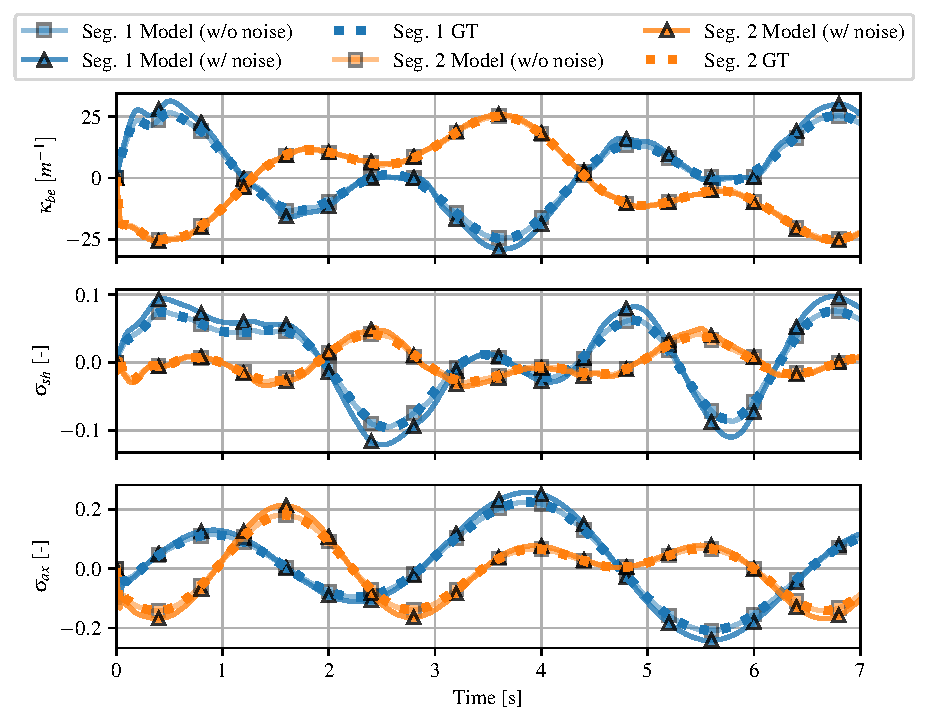
\includegraphics[width=0.49\textwidth, trim={5 5 5 5}]{pcsregression/figures/pcs_ns-2/ns-2_configuration_plots.pdf}\label{fig:pcsregression:predict_ns-2:subfig-1}}
    % Second subfigure
    \subfigure[End-effector pose]{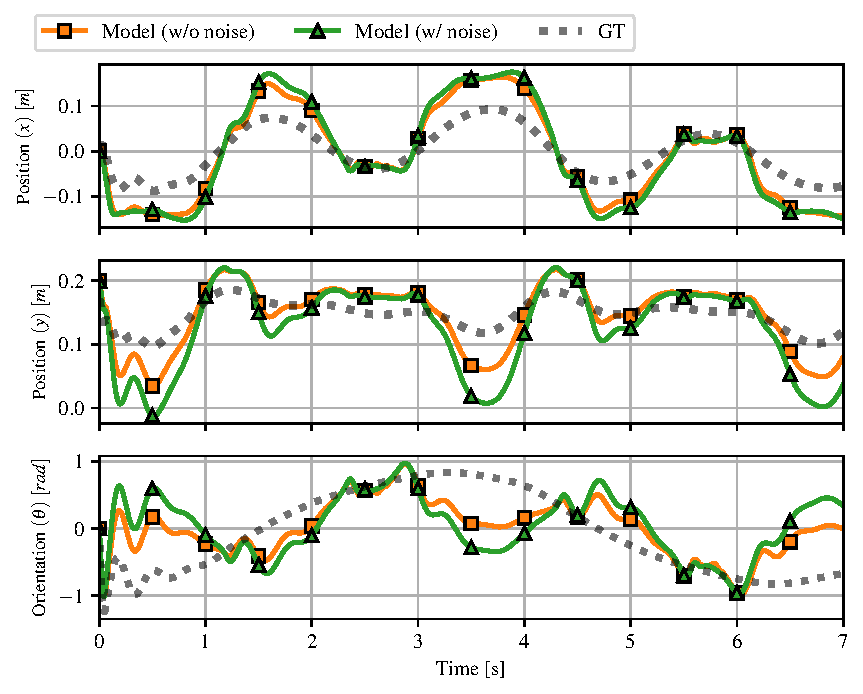
\includegraphics[width=0.47\textwidth, trim={5 5 5 5}]{pcsregression/figures/pcs_ns-2/ns-2_ee_comparison_plots.pdf} \label{fig:pcsregression:predict_ns-2:subfig-2}}

    \caption{Verification of the dynamical model with noise for a two-segment PCS soft robot (\emph{Case 2}). The dotted lines denote the ground-truth (GT) trajectory. For the configuration plot, blue lines refer to the first segment, while orange lines are associated with the second segment. For the end-effector pose plot, the orange and green lines mark the models trained with and without noise, respectively.}
    \label{fig:pcsregression:predict_ns-2}
\end{figure}
% \begin{figure}[htbp]
%     \centering
%     % First subfigure
%     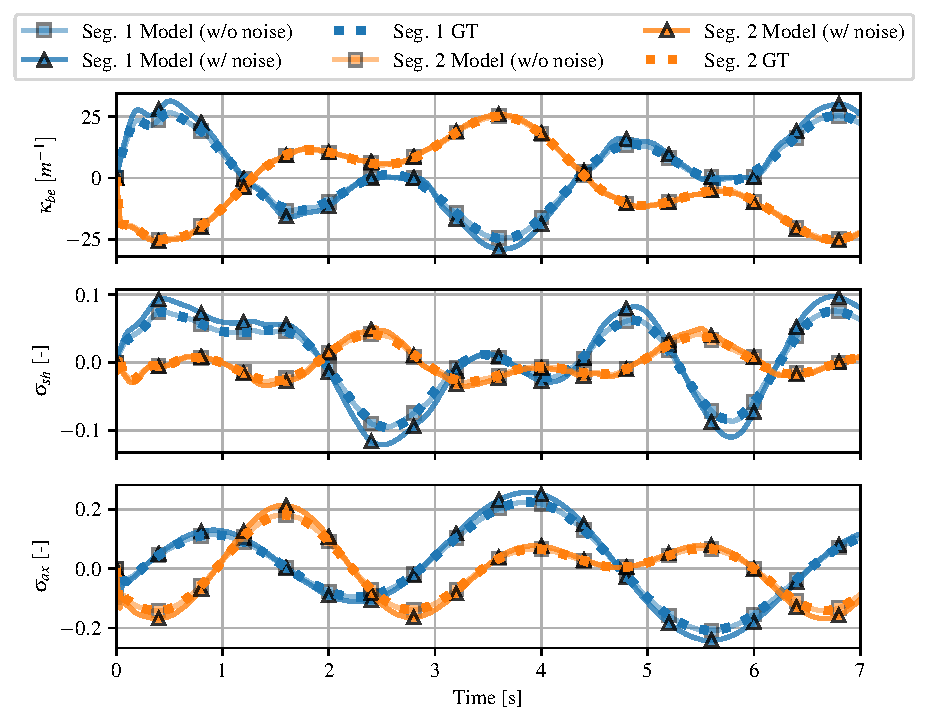
\includegraphics[width=0.8\columnwidth, trim={5 5 5 5}]{pcsregression/figures/pcs_ns-2/ns-2_configuration_plots.pdf}\label{fig:pcsregression:predict_ns-2_subfig-1}

%     \caption{Verification of the dynamical model with noise for a two-segment PCS soft robot (\emph{Case 2}). The dotted lines denote the ground-truth (GT) trajectory. The blue lines refer to the first segment, while the orange lines are associated with the second segment. % For the end-effector pose plot, the orange and green lines mark the models trained with and without noise, respectively.
%     }
%     \label{fig:pcsregression:predict_ns-2}
% \end{figure}

\begin{figure*}[ht]
    \centering
    \subfigure[$t=\SI{0.0}{s}$]{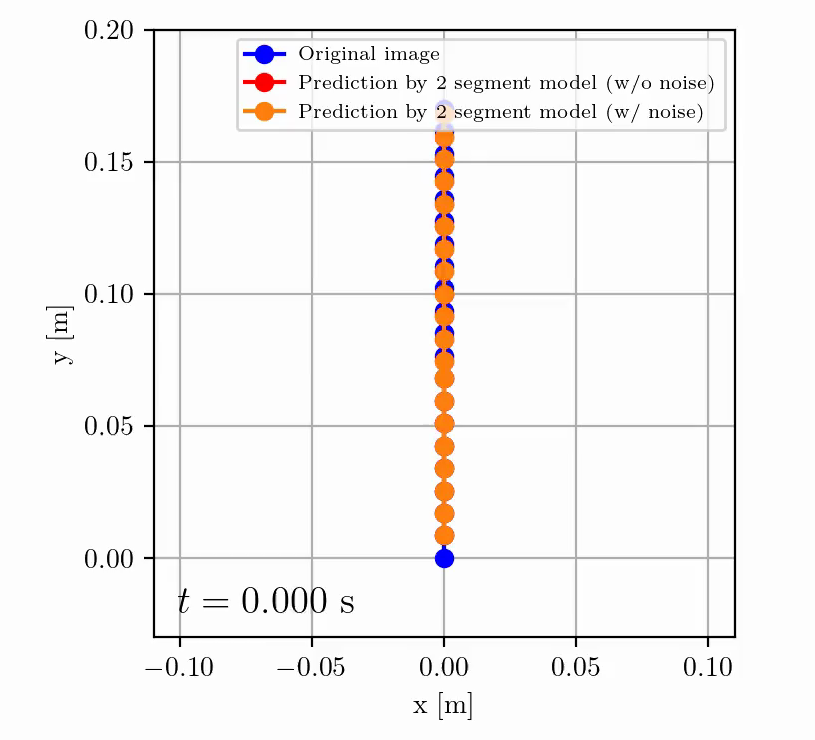
\includegraphics[width=0.320\textwidth,trim={5 5 5 5}]{pcsregression/figures/pcs_ns-2/sequence_of_stills/ns-2_task_space_animation_noise_comp_0.00.png}}
    \subfigure[$t=\SI{1.4}{s}$]{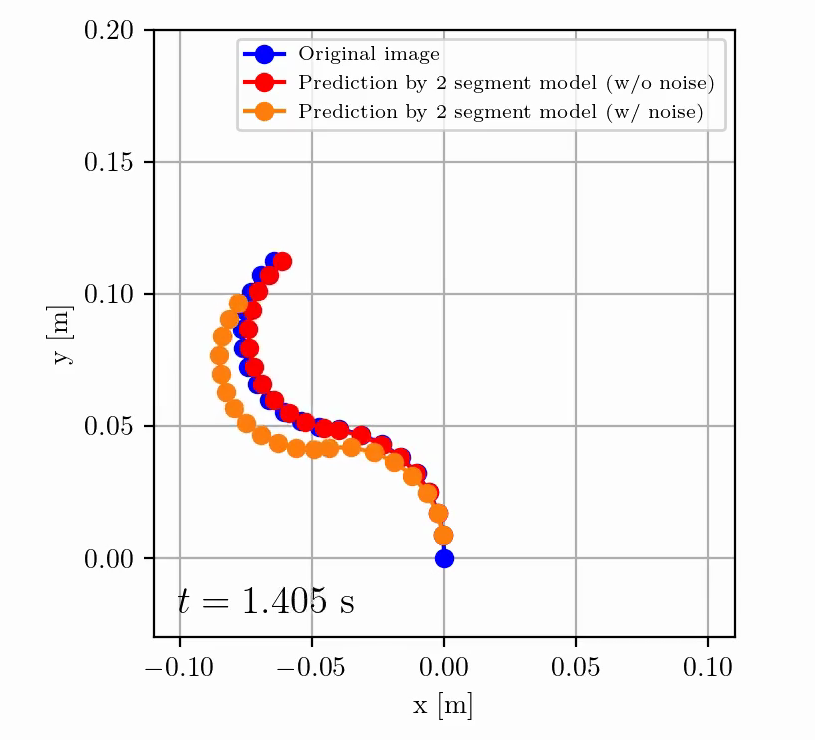
\includegraphics[width=0.320\textwidth,trim={5 5 5 5}]{pcsregression/figures/pcs_ns-2/sequence_of_stills/ns-2_task_space_animation_noise_comp_1.40.png}}
    \subfigure[$t=\SI{2.8}{s}$]{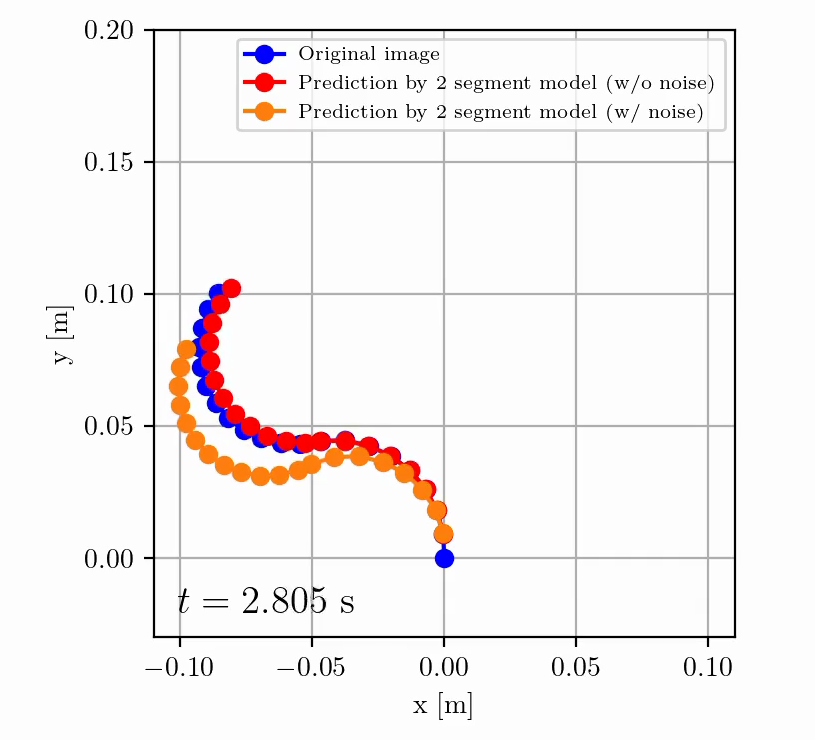
\includegraphics[width=0.320\textwidth,trim={5 5 5 5}]{pcsregression/figures/pcs_ns-2/sequence_of_stills/ns-2_task_space_animation_noise_comp_2.80.png}}\\
    \subfigure[$t=\SI{4.2}{s}$]{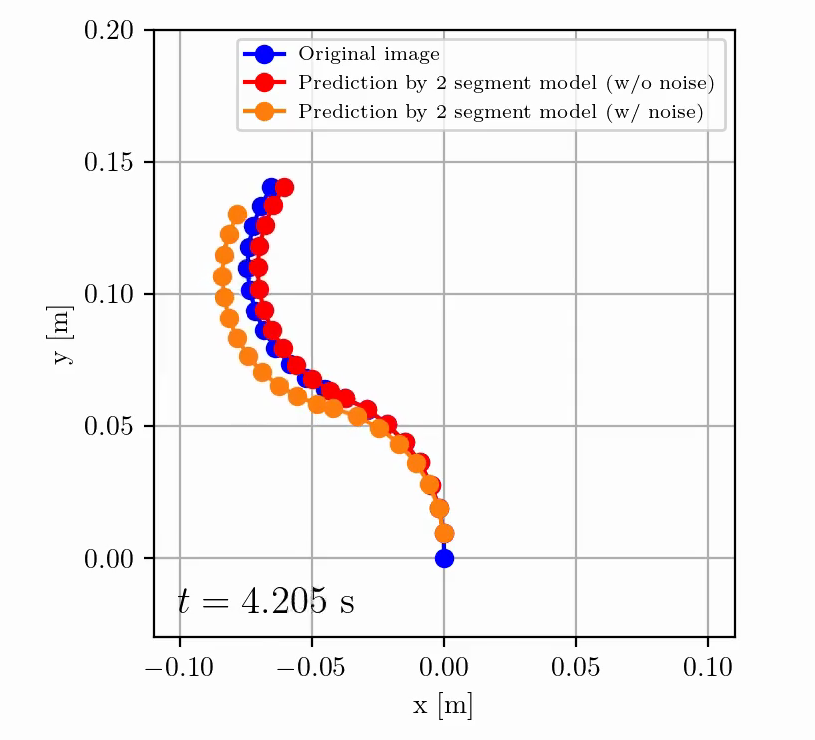
\includegraphics[width=0.320\textwidth,trim={5 5 5 5}]{pcsregression/figures/pcs_ns-2/sequence_of_stills/ns-2_task_space_animation_noise_comp_4.21.png}}
    \subfigure[$t=\SI{5.6}{s}$]{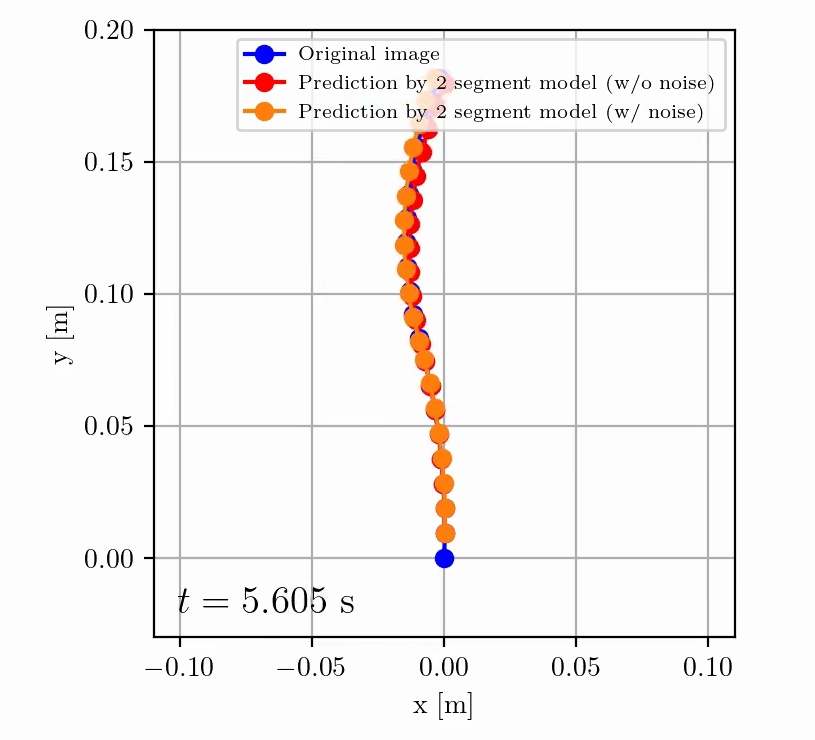
\includegraphics[width=0.320\textwidth,trim={5 5 5 5}]{pcsregression/figures/pcs_ns-2/sequence_of_stills/ns-2_task_space_animation_noise_comp_5.61.png}}
    \subfigure[$t=\SI{7.0}{s}$]{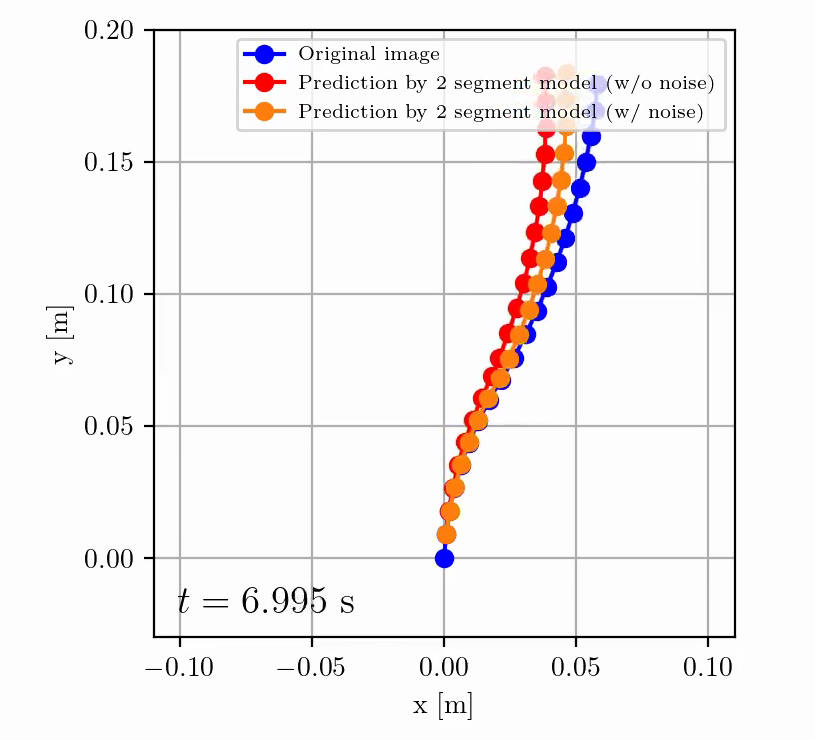
\includegraphics[width=0.320\textwidth,trim={5 5 5 5}]{pcsregression/figures/pcs_ns-2/sequence_of_stills/ns-2_task_space_animation_noise_comp_7.00.png}}
    \caption{Sequence of stills for the test rollout of the regressed dynamic model trained on the two-segment \gls{PCS} dataset (\emph{Case 2}). The blue and red dots represent the ground truth and estimated shape of the soft robot, respectively. The orange line represents the shape estimated by a model trained on a training set with added measurement noise.}\label{fig:pcsregression:still_seq}
\end{figure*}
% \begin{figure*}[htbp]
% \centerline{\includegraphics[width=\textwidth]{pcsregression/figures/sequence_stills.pdf}}
% \caption{Sequence of stills for the validation trajectory of Case 1, with the model trained without noisy data. The blue dots represent the actual position of the soft robot, while the red dots mark the position of the learned dynamic model.}
% \label{fig:pcsregression:still_seq}
% \end{figure*}

% The model trained without noise reports great accuracy, with an end-effector position error of $5.22\, \mathrm{mm}$ (3\% of the robot's length) and an orientation error of $0.14\,\mathrm{rad}$. An expected performance degradation is noticed for the model trained with noisy data, particularly for the end-effector position, which sees the error increase to $1.68\, \mathrm{cm}$. This raises some considerations for implementations in real-world scenarios where measurement noise is inevitable. Thus, while the model still gives reasonable predictions to moderate levels of noise, applying noise filtering techniques during the kinematic fusion process (where the measured task-space poses are converted into configurations) could help improve the robustness of the method to higher levels of noise.
% \subsubsection{Case 4}
% To evaluate the strain sparsification step in the dynamic regression, we used a one-segment PCS manipulator similar to Case 1, but with the shear strain stiffness set to a high value to simulate a scenario with minimal shear displacement.

% After running the regression, the obtained estimated stiffness was
% \begin{align}
%     \hat{K} = \mathrm{diag} \begin{bmatrix}
%     1.07\times 10^{-3} & 1.20 \times 10^3 & 1.16\times10^1 
% \end{bmatrix}\,.
% \end{align}
% Comparing the values with the maximum stiffness in \eqref{eq:pcsregression:max_stiffness}, the second entry, correspondent to the shear stiffness, is above the maximum value. Given this, the shear strain is neglected from the configuration vector and we update the Lagrangian basis functions through \eqref{eq:pcsregression:update_basis_fcns}, which results in a reduction from 51 to 27 basis functions. The Euler-Lagrange basis functions are also updated through \eqref{eq:pcsregression:update_basis_fcns_euler_lagrange}. The regression is again performed to estimate the 29 coefficients (27 plus the remaining 2 damping terms). In this case, the estimated stiffness is
% \begin{align}
%     \hat{K} =\mathrm{diag} \begin{bmatrix}
%         \hat{k}_{\text{be}} & \hat{k}_{\text{ax}}   
%         \end{bmatrix} = \mathrm{diag}\begin{bmatrix}
%             1.21\times 10^{-3} & 1.17 \times 10^1 
%         \end{bmatrix} \,,
% \end{align}
% which no longer requires additional sparsification.
% Figure \ref{fig:pcsregression:predict_ns-1_high_shear} shows the results for rolling out this dynamic model over the sinusoidal trajectory. To observe the impact of neglecting the shear strain, we additionally plot the end-effector pose for the case where shear was still considered. The end-effector errors for this comparison are also reported in the last two rows of Table \ref{tab:pcsregression:dyn_results}.


% \begin{figure}[htbp]
%     \centering
%     % First subfigure
%     \subfigure[Configurations]{\includegraphics[width=0.46\textwidth]{pcsregression/figures/ns-1_configuration_plots_high_shear.pdf}\label{fig:pcsregression:predict_ns-1_high_shear_subfig-1}}
%     % Second subfigure
%     \subfigure[End-effector pose]{\includegraphics[width=0.465\textwidth]{pcsregression/figures/ns-1_ee_comparison_plots_shear_vs_no_shear.pdf}\label{fig:pcsregression:predict_ns-1_high_shear_subfig-2}}

%     \caption{Verification of the model obtained for Case 4 on a sinusoidal trajectory. The dotted line denotes the ground-truth trajectory, while the green and orange lines correspond to the models trained with and without noise, respectively.}
%     \label{fig:pcsregression:predict_ns-1_high_shear}
% \end{figure}

\begin{figure}[ht]
    \centering
    % First subfigure
    \subfigure[Case 4: Configurations]{\includegraphics[width=0.47\linewidth, trim={5 5 5 5}]{pcsregression/figures/pcs_ns-1_high_shear_stiffness/ns-1_configuration_plots_high_shear.pdf}\label{fig:pcsregression:predict_ns-1_high_shear_subfig-1}}
    % Second subfigure
    \subfigure[Case 4: End-effector pose]{\includegraphics[width=0.49\linewidth, trim={5 5 5 5}]{pcsregression/figures/pcs_ns-1_high_shear_stiffness/ns-1_ee_comparison_plots_shear_vs_no_shear.pdf}\label{fig:pcsregression:predict_ns-1_high_shear_subfig-2}}\\
    \subfigure[Case 5: Configurations]{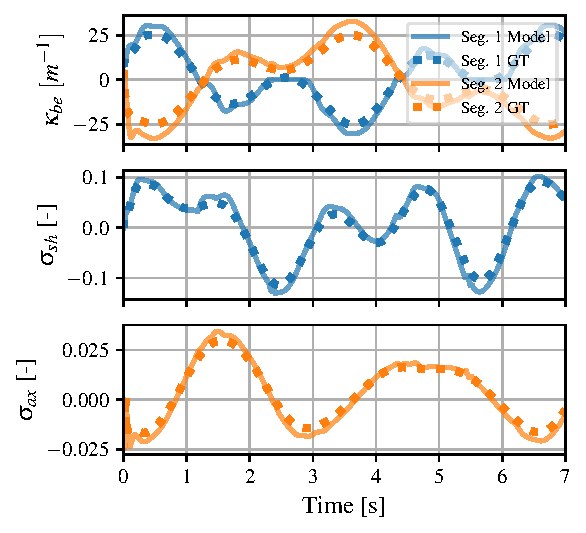
\includegraphics[width=0.49\linewidth, trim={5 5 5 5}]{pcsregression/figures/pcs_ns-2_high_stiffness/ns-2_configuration_plots.pdf}\label{fig:pcsregression:predict_ns-2_high_stiffness_subfig-1}}
    \subfigure[Case 5: End-effector pose]{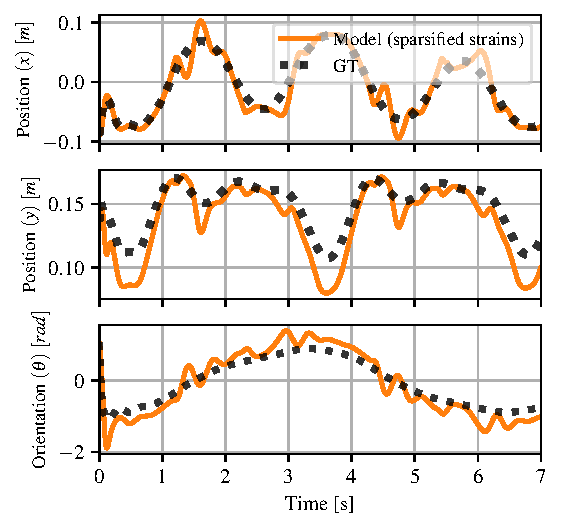
\includegraphics[width=0.47\linewidth, trim={5 5 5 5}]{pcsregression/figures/pcs_ns-2_high_stiffness/ns-2_ee_comparison_plots.pdf}\label{fig:pcsregression:predict_ns-2_high_stiffness_subfig-2}}

    \caption{Verification of the strain sparsification algorithm on a one-segment \gls{PCS} robot with shear modulus (\emph{Case 4}) and on a two-segment \gls{PCS} robot where the \nth{1} segment exhibits high axial stiffness and the second segment high shear stiffness. We roll out both the ground truth (dotted line) and the learned (solid line) model dynamics from the same initial condition and for a given sinusoidal actuation sequence.  Verification of the model obtained for Case 4 on a sinusoidal trajectory. The dotted line denotes the ground-truth trajectory, while the green and orange lines correspond to the models trained with and without noise, respectively.
    % For \emph{Cases 4}, the strain sparsification algorithm decides to neglect shear strains. Therefore, we only the bending and axial strain dynamics are considered during the rollout. The same applies to \emph{Case 5}, where the strain sparsification chooses to neglect the axial strain of the first segment and the shear strain of the segment.
    }
    \label{fig:pcsregression:results:strain_sparsification}
\end{figure}

% Figure \ref{fig:pcsregression:predict_ns-1_high_shear_subfig-1} shows that, despite discarding the shear strain, the model can still accurately predict the behaviour of the remaining bending and axial strains. Interestingly, the model without shear strain performs similarly, even slightly better, in terms of end-effector accuracy, compared to the model that includes all strains. Although it could be expected that the higher order model would perform better, a possible explanation is that, with fewer basis functions parametrizing the Lagrangian, the regressed coefficients for the remaining strains are more accurately estimated.

\begin{figure}[ht]
    \centering

    \subfigure[Train: Marker $s=\SI{68}{mm}$]{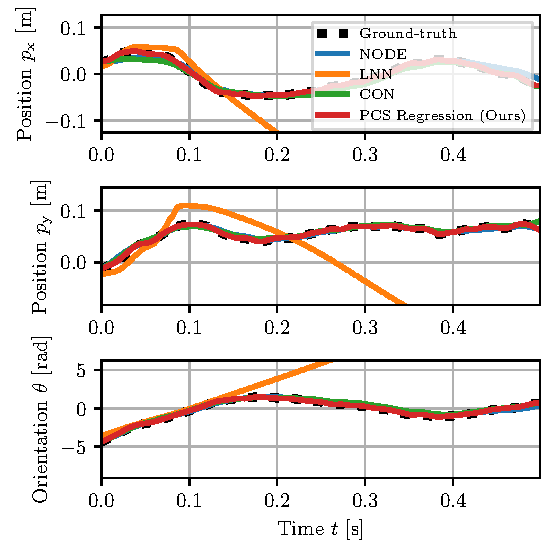
\includegraphics[width=0.49\textwidth]{pcsregression/figures/pcs_ns-2_with_baselines/rollout_train_marker_8.pdf}}
    \subfigure[Train: Marker $s=\SI{119}{mm}$]{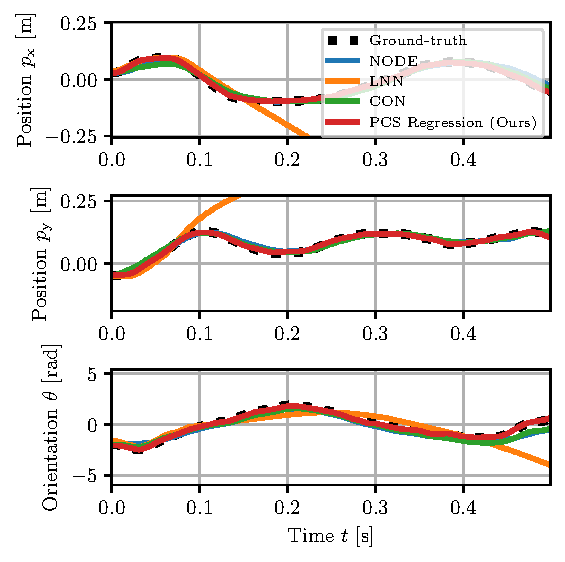
\includegraphics[width=0.49\textwidth]{pcsregression/figures/pcs_ns-2_with_baselines/rollout_train_marker_14.pdf}}\\
    \subfigure[Train: Marker $s=\SI{170}{mm}$ (EE)]{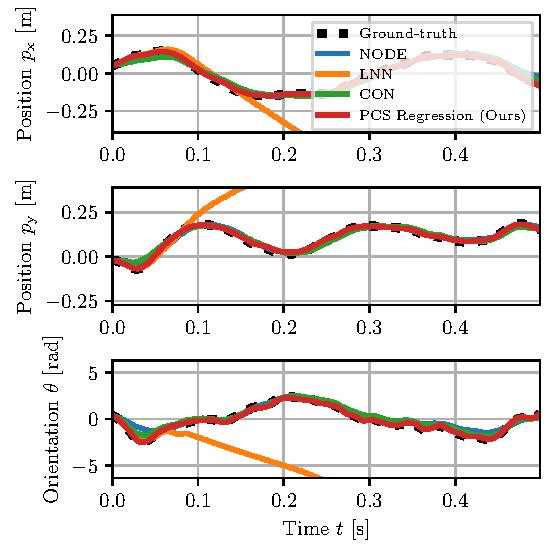
\includegraphics[width=0.49\textwidth]{pcsregression/figures/pcs_ns-2_with_baselines/rollout_train_marker_20.pdf}}
    \subfigure[Train: Actuation torques]{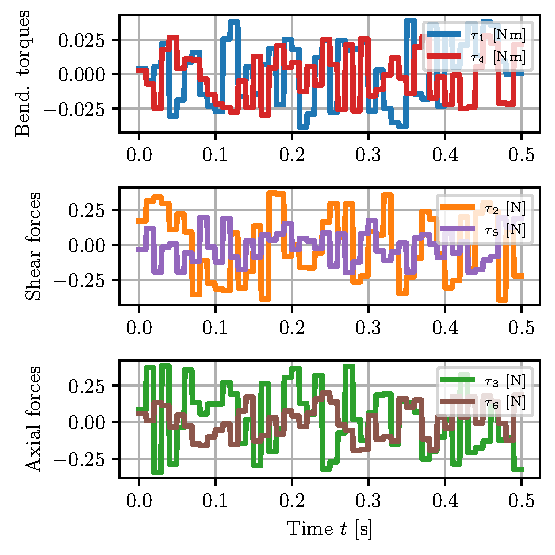
\includegraphics[width=0.49\textwidth]{pcsregression/figures/pcs_ns-2_with_baselines/torque_train.pdf}}

    \caption{Benchmarking of the proposed method against various machine learning baselines on a PCS soft robot consisting of two segments (\emph{Case 2}) on the \textbf{train dataset}: We train the baseline methods on the dynamical evolution of the Cartesian SE(2) poses of three \emph{markers} distributed over the backbone of the soft robot with a total length of \SI{170}{mm}. The upper and lower rows visualize the rollout of all methods on the training and the test set, respectively. The first three columns show the evolution of each of the three markers, where the last marker represents the end-effector. The last column displays the actuation torques that were used to generate the datasets.}
    \label{fig:pcsregression:dynamics_pcs_ns-2_with_baselines:training}
\end{figure}
\begin{figure}[ht]
    \centering
    \subfigure[Test: Marker $s=\SI{68}{mm}$]{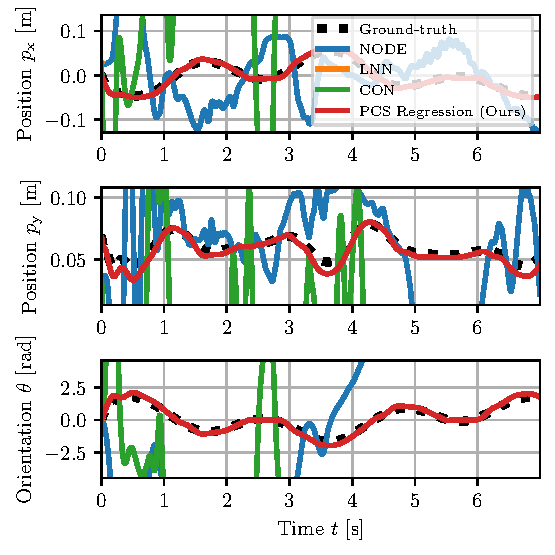
\includegraphics[width=0.49\textwidth]{pcsregression/figures/pcs_ns-2_with_baselines/rollout_val_marker_8.pdf}}
    \subfigure[Test: Marker $s=\SI{119}{mm}$]{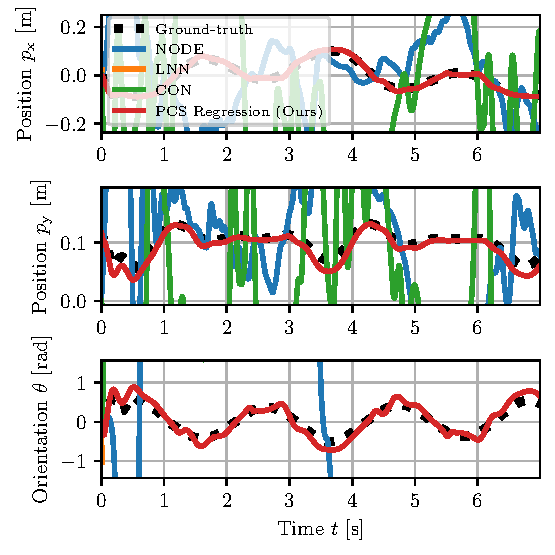
\includegraphics[width=0.49\textwidth]{pcsregression/figures/pcs_ns-2_with_baselines/rollout_val_marker_14.pdf}}\\
    \subfigure[Test: Marker $s=\SI{170}{mm}$ (EE)]{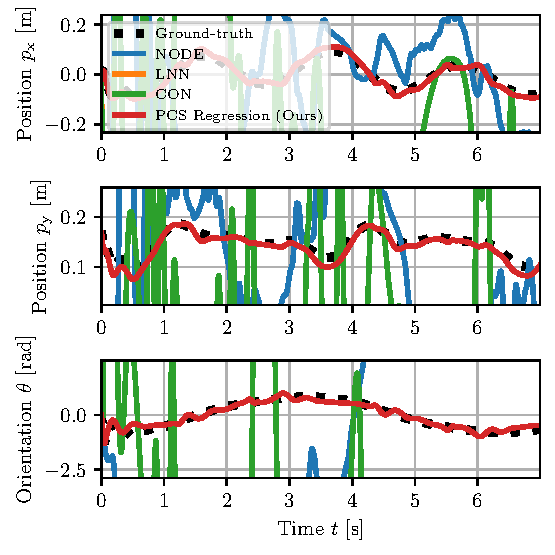
\includegraphics[width=0.49\textwidth]{pcsregression/figures/pcs_ns-2_with_baselines/rollout_val_marker_20.pdf}}
    \subfigure[Test: Actuation torques]{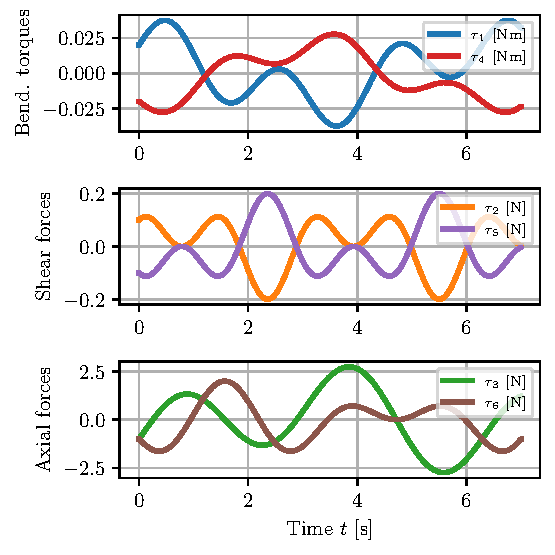
\includegraphics[width=0.49\textwidth]{pcsregression/figures/pcs_ns-2_with_baselines/torque_val.pdf}}

    \caption{Benchmarking of the proposed method against various machine learning baselines on a PCS soft robot consisting of two segments (\emph{Case 2}) on the \textbf{test dataset}: We train the baseline methods on the dynamical evolution of the Cartesian SE(2) poses of three \emph{markers} distributed over the backbone of the soft robot with a total length of \SI{170}{mm}. The upper and lower rows visualize the rollout of all methods on the training and the test set, respectively. The first three columns show the evolution of each of the three markers, where the last marker represents the end-effector. The last column displays the actuation torques that were used to generate the datasets.}
    \label{fig:pcsregression:dynamics_pcs_ns-2_with_baselines:test}
\end{figure}
% \begin{figure}[hbt]
%     \centering

%     \subfigure[Train: End-effector poses]{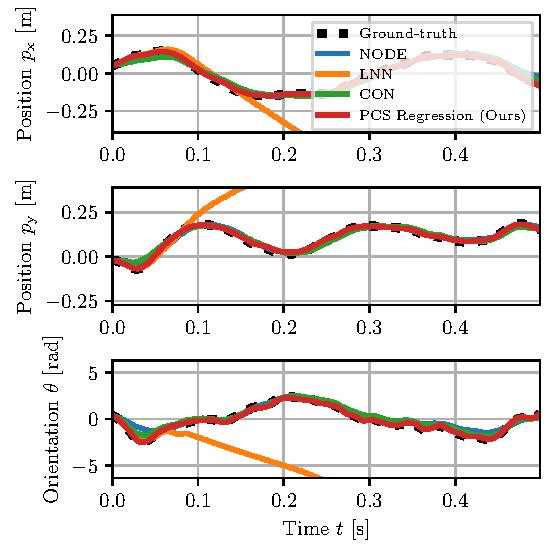
\includegraphics[width=0.49\columnwidth]{pcsregression/figures/pcs_ns-2_with_baselines/rollout_train_marker_20.pdf}}
%     \subfigure[Train: Actuation torques]{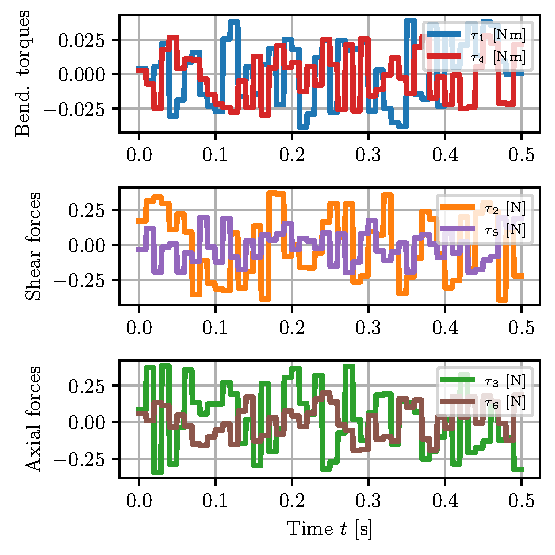
\includegraphics[width=0.49\columnwidth]{pcsregression/figures/pcs_ns-2_with_baselines/torque_train.pdf}}\\
%     \subfigure[Test: End-effector poses]{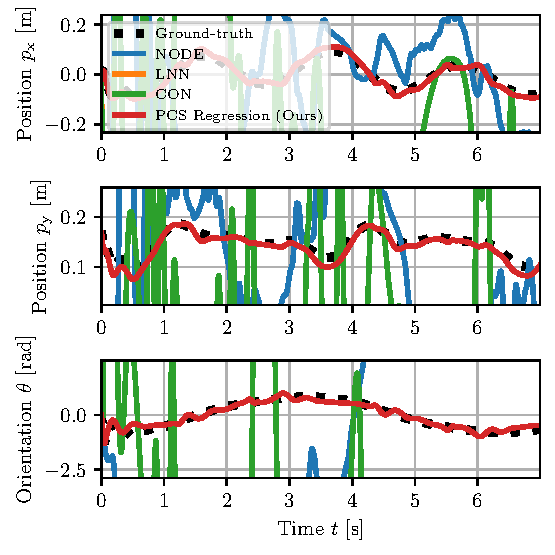
\includegraphics[width=0.49\columnwidth]{pcsregression/figures/pcs_ns-2_with_baselines/rollout_val_marker_20.pdf}}
%     \subfigure[Test: Actuation torques]{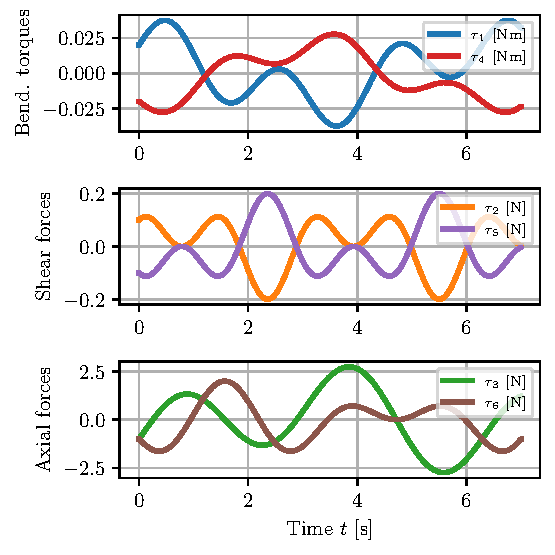
\includegraphics[width=0.49\columnwidth]{pcsregression/figures/pcs_ns-2_with_baselines/torque_val.pdf}}

%     \caption{Benchmarking of the proposed method against various machine learning baselines on a PCS soft robot consisting of two segments (\emph{Case 2}): We train the baseline methods on the dynamical evolution of the Cartesian SE(2) poses of three \emph{markers} distributed over the backbone of the soft robot with a total length of \SI{170}{mm}. The upper and lower rows visualize the rollout of all methods on the training and the test set, respectively. The first column shows the evolution end-effector pose. The last column displays the actuation torques that were used to generate the datasets.}
%     \label{fig:pcsregression:dynamics_pcs_ns-2_with_baselines}
% \end{figure}

\begin{table}[htbp]
\centering
%\renewcommand{\arraystretch}{1.3} % Increase space between rows
\caption{Results for learning dynamics of a two-segment PCS soft robot (Case 2). We report the position ($e_\mathrm{p}^\mathrm{body}$) and orientation ($e_\theta^\mathrm{body}$) metrics that capture the mean shape error averaged over all time steps. The shape error is computed by considering the dynamical evolution of three marker poses with $s_j \in \{ 68, 119, 170 \}$~\si{mm}. We report the metrics for a rollout of the dynamics on both a \SI{0.5}{s} sequence on the training set and the entire (i.e., \SI{7}{s}) test set.}
\label{tab:pcsregression:dynamics_pcs_ns-2_with_baselines}
\setlength\tabcolsep{3pt}
\begin{small}
\begin{tabular}{c r r r r}
    \toprule
    \textbf{Method} & \textbf{Train} $\mathbf{e_\mathrm{p}^\mathrm{body}}$ & \textbf{Train} $\mathbf{e_\theta^\mathrm{body}}$ & \textbf{Test} $\mathbf{e_\mathrm{p}^\mathrm{body}}$ & \textbf{Test} $\mathbf{e_\theta^\mathrm{body}}$\\
    \midrule
    \gls{NODE} & \SI{10.4}{mm} & \SI{0.27}{rad} & \SI{245.6}{mm} & \SI{12.22}{rad}\\
    \gls{LNN}~\citep{liu2024physics} & \SI{550.8}{mm} & \SI{5.16}{rad} & $\infty$ & $\infty$\\
    \gls{CON}~\citep{stolzle2024input} & \SI{12.9}{mm} & \SI{0.24}{rad} & \SI{789.5}{mm} & \SI{29.49}{rad}\\
    \textbf{PCS Regression (Ours)} & $\mathbf{3.1}$~\si{mm} & $\mathbf{0.04}~\si{rad}$ & $\mathbf{9.8}$~\si{mm} & $\mathbf{0.13}~\si{rad}$\\
    \bottomrule
\end{tabular}
\end{small}
\end{table}

\subsection{Benchmarking of Identified Dynamics against ML Baselines}
We benchmark the derived dynamical model of \emph{Case 2} (i.e., a two-segment planar \gls{PCS} soft robot) against several models trained using machine learning approaches. Specifically, we consider various learning-based approaches that range from completely data-driven (e.g., \gls{NODE}) over approaches that take into account the structure of Lagrangian systems (e.g., \gls{LNN}, \gls{CON}).
% To keep the comparison fair, we define the task as learning the dynamical evolution of the backbone without any access to prior information about the kinematics (e.g., no knowledge about number of segments, length of each segment, active strains, etc.).
To keep the comparison fair, we define the inputs for all methods as the Cartesian poses $\chi_j \in \mathbb{R}^3$ and the corresponding time derivative $\dot{\chi}_j$ of $N$ discrete \emph{markers} along the backbone. Furthermore, we also provide the actuation torques $\tau \in \mathbb{R}^6$ as a dynamic model input. Therefore, the total model input exhibits a dimensionality of $\mathbb{R}^{6N + 6}$. The task of the dynamic model is to predict the acceleration $\ddot{\chi}(k) \in \mathbb{R}^{3N}$. % (\gls{NODE}, \gls{CON}, \gls{LNN}). % or next state $(\chi(k+1), \dot{\chi}(k+1)) \in \mathbb{R}^{18}$ (\gls{LSTM}) of all markers.
We tried supplying all $21$ markers, which our method also has access to, to the baseline approaches. However, this proved to be infeasible as the problem would become too high-dimensional in terms of the number of inputs and outputs, and the baseline approaches would overfit the training set. Therefore, we settled to give the baseline methods access to the pose measurements of $N=3$ markers distributed along the backbone of the robot at $s_j \in \{ 68, 119, 170 \}$~\si{mm}, where $s=\SI{170}{mm}$ corresponds to the end-effector.

\paragraph{Implementation of Baseline Methods}
The \gls{NODE} is parametrized by a six-layer \gls{MLP} with hidden dimension $256$ and hyperbolic tangent activation function that predicts based on the input $(\chi(t), \dot{\chi}(t), \tau(t))$ the acceleration $\ddot{\chi}$. We remark that with this strategy, we already infuse the prior knowledge that the time derivative of the pose is the velocity, which would not be the case in a naive implementation of a \gls{NODE}.
\glspl{CON}~\citep{stolzle2024input} allow for learning of (latent) dynamics of Lagrangian systems with strong stability guarantees (global asymptotic stability / input-to-state stability) by leveraging a network of damped harmonic oscillators that are coupled by a hyperbolic potential. In order to allow for arbitrary placement of the global asymptotically stable equilibrium point, we learn a linear coordinate transformation into the latent coordinates $z = W \chi + b \in \mathbb{R}^9$, $\dot{z} = W \dot{\chi}$. % After the latent acceleration $\ddot{z}$ is predicted by the \gls{CON} network, we can project it back into Cartesian space as $\ddot{\chi} = W^{-1} \ddot{z}$. 
% We parametrize the actuation to oscillator forcing mapping $V(\tau) \in \mathbb{R}^{6 \times 9}$ with a five-layer MLP with hidden dimension $16$ (\texttt{tanh} activation).
\glspl{LNN} learn the components of the Lagrangian $\mathcal{L}(\chi, \dot{\chi}) = \frac{1}{2} \dot{\chi}^\top M(\chi) \dot{\chi} - \mathcal{U}(\chi)$ such as the mass matrix $M(\chi) \succ 0 \in \mathbb{R}^{9 \times 9}$, the potential energy $\mathcal{U}(\chi) \in \mathbb{R}$, the damping matrix $D \succeq 0 \in \mathbb{R}^{9 \times 9}$ and the actuation matrix $A \in \mathbb{R}^{6 \times 9}$ and subsequently derive the \gls{EOM} as $M(\chi) \ddot{\chi} + \frac{\partial \mathcal{L}}{\partial \chi \partial \dot{\chi}} \dot{\chi} + \frac{\partial \mathcal{U}}{\partial \chi} + D \dot{\chi} = A \tau$ using autodifferentiation.
We regard $A$ and $D$ as trainable weights and parametrize $M(\chi)$ and $\mathcal{U}(\chi)$ with six-layer \glspl{MLP} with hidden dimension $256$ (softplus activation). We leverage the Cholesky decomposition to make sure that $M(\chi), D \succ 0$.

\paragraph{Training}
% We split off the last \SI{20}{\percent} of the training set trajectory as the validation set.
% Analog to how the dynamic regression of our proposed method is implemented, the natural way would be to train the baseline methods (e.g., \gls{NODE}, \gls{CON}, \gls{LNN}) to directly predict the acceleration $\hat{\ddot{\chi}}(t)$ for every dataset input tuple $(\chi(k), \dot{\chi}(k), \tau(k))$.
% Then, we would apply a supervised training loss (e.g., \gls{MSE}) between the predicted acceleration and the corresponding label $\ddot{\chi}(k)$, which is generated by numerically differentiating the pose trajectory.
% However, we found that even if the baseline models would accurately predict the accelerations on the validation loss, we would perform badly or even become unstable when rolled out over a mid-to-long time horizon (i.e., longer than approx. \SI{0.1}{s}).
% Therefore, even though this is not done for our proposed method, we additionally roll out the trajectories during training over a horizon of \SI{0.3}{s} and add loss terms that compute the \gls{MSE} error between the predicted states $(\hat{\chi}(k+r), \hat{\dot{\chi}}(k+r))$ and the training set states $(\chi(k+r), \dot{\chi}(k+r))$, where $r$ is the index of the rollout step.
The first loss term is a \gls{MSE} between the predicted $\hat{\ddot{\chi}}(k)$ and actual acceleration $\ddot{\chi}(k)$. Additionally, we roll out the trajectories over a horizon of \SI{0.3}{s} and add loss terms that compute the \gls{MSE} error between the predicted states $(\hat{\chi}(k+r), \hat{\dot{\chi}}(k+r))$ and the labels $(\chi(k+r), \dot{\chi}(k+r))$, where $r$ is the index of the rollout step.
As training \glspl{LNN} is computationally very demanding due to the need to differentiate w.r.t. both inputs and neural network parameters, we had to reduce the training rollout horizon. % restrict the horizon to \textcolor{orange}{\SI{0.01}{s}}.

\paragraph{Results}
We present the benchmarking results in Fig.~\ref{fig:pcsregression:dynamics_pcs_ns-2_with_baselines:training} (evaluation on the training set) and Fig.~\ref{fig:pcsregression:dynamics_pcs_ns-2_with_baselines:test} (evaluation on the test set). Quantitative error metrics are provided in Table~\ref{tab:pcsregression:dynamics_pcs_ns-2_with_baselines}.
We report the performance for rollouts on both the training and the test set.
All methods, except for \gls{LNN}, are able to predict the Cartesian-space evolution of the markers attached to the soft robot backbone decently accurately over the training set trajectory. Still, the our proposed method exhibits an \SI{70}{\percent} to \SI{80}{\percent} lower error than \gls{NODE} and \gls{CON}~\citep{stolzle2024input}. As \gls{LNN} does not exhibit any stability guarantees and it is trained on a relatively short horizon, it diverges from the ground-truth trajectory after roughly \SI{0.15}{s}.
As shown in panels (d) of Figs.~\ref{fig:pcsregression:dynamics_pcs_ns-2_with_baselines:training} and \ref{fig:pcsregression:dynamics_pcs_ns-2_with_baselines:test}, the axial actuation forces on the validation set are one order of magnitude higher than in the training set. Therefore, these axial forces can be considered to be out-of-distribution for the trained models. Our proposed method is amazingly able to still exhibit very good performance, while all baseline methods are no longer able to predict the dynamic evolution of the system. \gls{LNN} even becomes fully unstable after a few milliseconds, and we are, therefore, not able to report test errors for this method.

\begin{figure}[ht]
    \centering
    \subfigure[Bending strains]{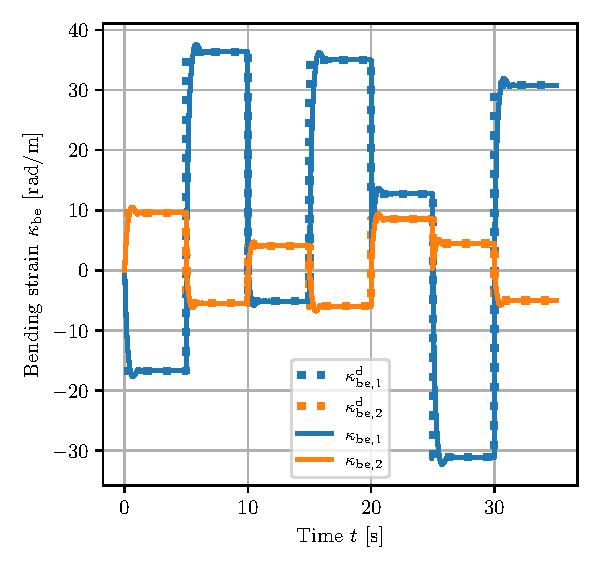
\includegraphics[width=0.4\columnwidth, trim={5 5 5 5}]{pcsregression/figures/control/setpoint_control_bending.pdf}}
    \subfigure[Linear strains]{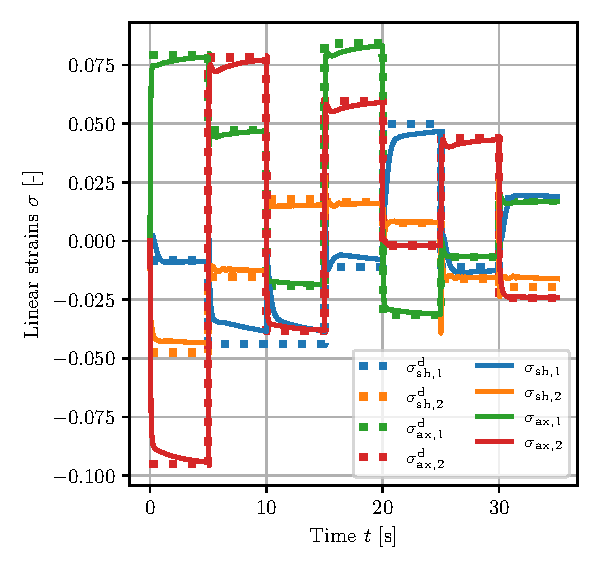
\includegraphics[width=0.4\columnwidth, trim={5 5 5 5}]{pcsregression/figures/control/setpoint_control_linear.pdf}}
    \caption{Demo of model-based control of a two-segment soft robot based on the learned dynamical model. We ask the controller to track a sequence of $7$ setpoints $q^\mathrm{d}\in \mathbb{R}^6$ which is denoted with dotted lines. The controller contains a feedforward and feedback term where the feedforward term compensates for the elastic and gravitational forces at the setpoint. 
    % We refer with $\kappa_{\mathrm{be},1}, \kappa_{\mathrm{be},2}$ to the bending strains of the first and second segment, respectively. Similarly, $\sigma_{\mathrm{sh},i}$ and $\sigma_{\mathrm{ax},i}$ represent the shear and axial strains.
    }
    \label{fig:pcsregression:results:control:pcs_ns-2}
\end{figure}

\subsection{Demonstration of Model-based Control}\label{sub:pcsregression:validation:model_based_control}
To demonstrate how the derived models can be used in a plug-and-play fashion for model-based control, we simulate the closed-loop dynamics of a simulated two-segment \gls{PCS} soft robot (\emph{Case 2}) with configuration $q \in \mathbb{R}^7$ under a P-satI-D+FF~\citep{della2023model, stolzle2024experimental, stolzle2024input} setpoint control policy
\begin{equation}
\begin{split}
    \tau(t, q) =& \: \underbrace{\hat{G}(q^\mathrm{d})+\hat{K}q^\mathrm{d}}_{\text{Learned feedforward term}} + \underbrace{K_\mathrm{p} \, (q^\mathrm{d} - q) - K_\mathrm{d} \, \dot{q} + K_\mathrm{i} \, e_\mathrm{int}(t) }_{\text{P-satI-D feedback term~\citep{pustina2022p}}},
\end{split}
\end{equation}
where $K_\mathrm{p}, K_\mathrm{i}, K_\mathrm{d} \in \mathbb{R}^{n \times n}$ are the proportional, integral, and derivative control gains, respectively.
The feedback control term is a PID-like controller with integral saturation~\citep{pustina2022p} and the dimensionless gain $\Upsilon \in \mathbb{R}$ which bounds the integral error at each time step to the interval $(-1, 1)$ and reduces the risk of instability for nonlinear systems
\begin{equation}
    e_\mathrm{int}(t, q) = \:  \int_0^t \tanh(\Upsilon (q^\mathrm{d}(t') - q(t'))) \: \mathrm{d}t',
\end{equation}
$\hat{G}(q) \in \mathbb{R}^{6}$ and $\hat{K} \in \mathbb{R}^{6 \times 6}$ are the estimated gravitational forces and stiffness matrix, respectively.
We simulate the closed-loop dynamics with a Tsitouras 5(4) integrator at a timestep of $\SI{0.05}{ms}$.
Please note that we use the ground-truth dynamics as a state transition function.
% After manual tuning, we select the control gains $K_\mathrm{p} = \mathrm{diag}(0.01, 0.5, 6, 0.01, 0.5, 6)$, $K_\mathrm{i} = \mathrm{diag}(0.06, 3, 36, 0.06, 3, 36)$, $K_\mathrm{d} = \mathrm{diag}(0.002, 0.1, 0.8, 0.002, 0.1, 0.8)$, and $\Upsilon = \mathrm{diag}(40, 0.1, 0.2, 40, 0.1, 0.2)$.

To verify that the learned model performs well within the model-based control policy, we create a sequence of $7$ randomly sampled setpoints $q^\mathrm{d}(k) \in \mathbb{R}^6$. % $} \in \mathcal{U}([-\SI{40}{rad \per m}, ], [])$.
The results in Fig.~\ref{fig:pcsregression:results:control:pcs_ns-2} show that the controller is able to effectively regulate a two-segment planar soft robot. %  that exhibits bending, shear, and axial strains.
The tracking of the bending strain reference is perfect. For the linear strains, we notice small errors in the feedforward term, but the integral control is able to compensate for them and drive the system toward the reference.
We stress that the structure and characteristics of the learned model enabled us to formulate the control policy in closed form easily, and we did not have to resort to techniques such as \gls{MPC} or \gls{RL} as it would be necessary for other model learning techniques (e.g., \glspl{LSTM}, \glspl{NODE}).